%\documentclass[a4paper,twoside,11pt]{article}
\documentclass[11pt, a4paper, oneside]{book}
\usepackage[utf8]{inputenc}

\usepackage{amsmath,amssymb,amsthm}
\usepackage{mathtools}

%\usepackage[style=authoryear]{biblatex}
\usepackage[citestyle=authoryear,bibstyle=authoryear,natbib]{biblatex}
\addbibresource{Sources.bib}

\usepackage{caption}
\usepackage{subcaption}
\usepackage{float}
\usepackage{array}
\usepackage{graphicx}
\usepackage{pgfplots}
\pgfplotsset{compat=1.13}
\usepackage{tikz}
\usetikzlibrary{arrows,patterns,calc,matrix,shapes}
\usetikzlibrary{arrows.meta}

\usepackage[margin=1in]{geometry}
\usepackage{placeins}
\usepackage{flafter}
\usepackage[doublespacing]{setspace}

\usepackage{lipsum}
\usepackage{titlesec}
\usepackage{nomencl}
\makenomenclature
\usepackage[toc,page]{appendix}
\usepackage{verbatim}
%\usepackage{algorithm2e}
%\usepackage[noend]{algpseudocode}
\usepackage{xcolor}
\usepackage[cache=false]{minted}
\usepackage{listings}
\lstdefinestyle{lua}{
    language=[5.1]Lua,
    basicstyle=\ttfamily,
    tabsize=3,
    showspaces=false,
    showstringspaces=false,
    numbers=left,
    numberstyle=\color{lightgray},
    numbersep=5pt,
    %backgroundcolor=\color{black!5},
    keywordstyle=\color{teal},
    stringstyle=\color{red},
    commentstyle=\color{black!50}
}
\usepackage{import}

\usepackage{booktabs}
\usepackage{fancyhdr}

%\usepackage{cleveref}
\usepackage{hyperref}

% headers and footers
\pagestyle{fancy}
\setlength{\headheight}{14pt}
\renewcommand{\chaptermark}[1]{\markboth{\chaptername\ \thechapter.\ #1}{}}
\renewcommand{\sectionmark}[1]{\markright{\thesection.\ #1}}
\lhead{\rightmark}
\rhead{\leftmark}

\newcommand{\numberthis}{\addtocounter{equation}{1}\tag{\theequation}}
%\newcommand{\nr}[1]{\refstepcounter{equation}\label{#1}\tag{\theequation}}

\newcommand{\Rmag}[1]{\left|#1\right|}
\newcommand{\Rvec}[1]{\mathbf{#1}}
\newcommand{\Rnvec}[1]{\Rvec{\hat{#1}}}
\newcommand{\Rmvec}[1]{\Rmag{\Rvec{#1}}}
\newcommand{\Rtvec}[1]{\overset{\tau}{\Rvec{#1}}}
\newcommand{\Rntvec}[1]{\overset{\tau}{\Rnvec{#1}}}
\newcommand{\Rdt}{\ensuremath{\delta t}}
\newcommand{\Rovercast}[2]{\overset{\mathclap{\scriptscriptstyle#2}}{#1}}
\newcommand{\Rclamp}[1]{\ensuremath{\text{clamp}\left(#1\right)}}
\newcommand{\Rthresh}[2]{\ensuremath{\left\rmoustache#1\right\lmoustache_{#2}}}
\newcommand{\Rraisemath}[2]{\raisebox{#1}{$\displaystyle#2$}}
\newcommand{\Reg}{{\itshape e.g.~}}
\newcommand{\Rarrowscale}{0.5pt}

\newcommand{\HIDE}[1]{\PackageWarning{HIDE}{Hidden text in \thesubsection}}
\newcommand{\TODO}[1]{\texttt{TODO}: \textit{#1}\PackageWarning{TODO}{"#1"}}

\pgfarrowsdeclare{Rrrow}{Rrrow}
{
  \pgfarrowsleftextend{-5.59\pgflinewidth}
  \pgfarrowsrightextend{4.5\pgflinewidth}
}
{
  \pgfpathmoveto{\pgfpoint{4.5\pgflinewidth}{0pt}} %Point5
  \pgfpathlineto{\pgfpoint{-0.63\pgflinewidth}{1.09\pgflinewidth}} %Point4
  \pgfpathlineto{\pgfpoint{-5.48\pgflinewidth}{3.06\pgflinewidth}} %Point3
  \pgfpathlineto{\pgfpoint{-5.59\pgflinewidth}{3.0\pgflinewidth}}%Point2
  \pgfpathlineto{\pgfpoint{-3.95\pgflinewidth}{0pt}} %Point1
  \pgfpathlineto{\pgfpoint{-5.59\pgflinewidth}{-3.0\pgflinewidth}}%Point8
  \pgfpathlineto{\pgfpoint{-5.48\pgflinewidth}{-3.06\pgflinewidth}}%Point7
  \pgfpathlineto{\pgfpoint{-0.63\pgflinewidth}{-1.09\pgflinewidth}}%Point6
  \pgfusepathqfill
}


% intro to neural networks (background/history)
% - biological
% - artificial intelligence
% - preceptron
% - backpropagation
% - other types of networks
%   - convolutional
%   - recurrent
% introduction to python
% - neural networks in python
%   - single layer boston
%   - multilayer boston
%   - xor
% - tensorflow and keras
%   - boston
%   - xor
%   - linear regression
%   - character regression
% <application>
% - prior work
% - application aims
% - mathematics
% - neural network
% - results
% conclusion

% ^ nice try

\begin{document}

\begin{titlepage}
\begin{center}
    \vspace{2cm}
    
\includegraphics[width = 6cm]{MMU_Logo_Colour.pdf}\\
    \textbf{\Large Faculty of Science and Engineering}\\
    \vspace{2cm}
    \textbf{\LARGE Alexander J. Johnson}\\
    \vspace{1cm}
    {\Large Mathematics}\\
    \vspace{1cm}
    \textbf{\LARGE Neural Networks with Python and TensorFlow}\\
    \vspace{1cm}
    {\Large\today}\\
    
    \vfill
    
    {\large School of Computing, Mathematics and Digital Technology}
\end{center}
\end{titlepage}

\addcontentsline{toc}{chapter}{Abstract}
\chapter*{Abstract}

Artificial Intelligence (AI) still remains as one of the greatest challenges in
scientific research to this date, but much progress in the field has been made
using artificial neural networks.
The design of artificial neural networks is loosely inspired by that of
biological brains, and serves as an expansion of an earlier concept called the
perceptron \citep{Rosenblatt:1958:Perceptron}.
By using multiple layers of these artificial neurons, we can form a highly
connected system that is referred to as a neural network,
these networks can then be trained on a large data set to predict the output
with high accuracy.

The range applications for neural networks is wide: they can be used to classify
data, predict future states of chaotic systems, apply stylisations to images,
or control physical/physically-based systems in real-time.

This project aims to cover the history of a wide range of artificial neural
networks and their applications.

\chapter*{Declaration}
With the exception of any statement to the contrary, all the material presented in this report is the result of my own efforts. In addition, no parts of this report are copied from other sources. I understand that any evidence of plagiarism and/or the use of unacknowledged third party materials will be dealt with as a serious matter.
\vspace{2cm}

Signed\vspace{-12pt}
\begin{center}
    
\includegraphics[width=150pt]{Signiture.jpg}\vspace{-25.6pt}\\
	\line(1,0){250}
\end{center}
\tableofcontents
\chapter{Introduction to Neural Networks}

%\TODO{Chapter: Introduction}

\section{Biological Neurons}

Biological neurons are electrically excitable cells that are found in almost all
animals.
These neurons can transmit and receive electrical signals to one another via
synaptic connections, which maybe either excitatory or inhibitory.
Any given neuron will be either active or inactive depending on whether or not
its input exceeds a threshold.
\rfig{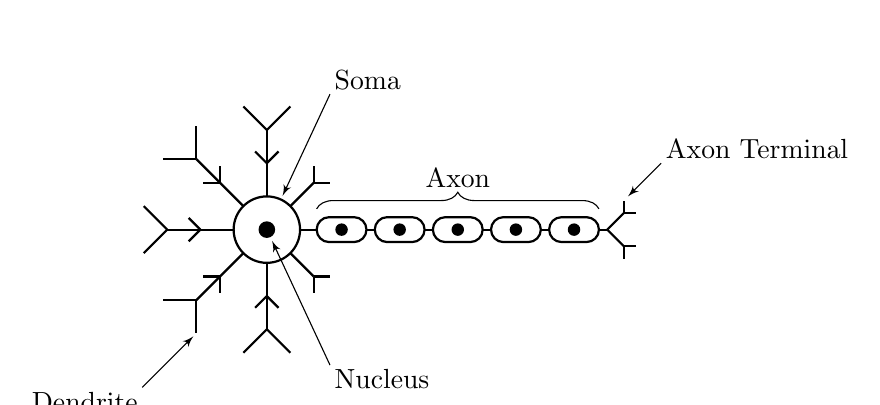
\begin{tikzpicture}%[x=1pt,y=1pt]
    \newlength{\rs}
    \setlength{\rs}{1.5pt}
    % Nucleus
    \fill (0\rs,0\rs) circle (2\rs);
    % Soma
    \draw[thick] (0\rs,0\rs) circle (8\rs);
    % Dendrite
    \draw[thick] ( 45:8\rs) -- ( 45:16\rs);
        \draw[thick] ( 45:16\rs) -- ++(  0:4\rs);
        \draw[thick] ( 45:16\rs) -- ++( 90:4\rs);
    \draw[thick] ( 90:8\rs) -- ( 90:24\rs);
        \draw[thick] ( 90:16\rs) -- ++( 45:4\rs);
        \draw[thick] ( 90:16\rs) -- ++(135:4\rs);
        \draw[thick] ( 90:24\rs) -- ++( 45:8\rs);
        \draw[thick] ( 90:24\rs) -- ++(135:8\rs);
    \draw[thick] (135:8\rs) -- (135:24\rs);
        \draw[thick] (135:16\rs) -- ++( 90:4\rs);
        \draw[thick] (135:16\rs) -- ++(180:4\rs);
        \draw[thick] (135:24\rs) -- ++( 90:8\rs);
        \draw[thick] (135:24\rs) -- ++(180:8\rs);
    \draw[thick] (180:8\rs) -- (180:24\rs);
        \draw[thick] (180:16\rs) -- ++(135:4\rs);
        \draw[thick] (180:16\rs) -- ++(225:4\rs);
        \draw[thick] (180:24\rs) -- ++(135:8\rs);
        \draw[thick] (180:24\rs) -- ++(225:8\rs);
    \draw[thick] (225:8\rs) -- (225:24\rs);
        \draw[thick] (225:16\rs) -- ++(180:4\rs);
        \draw[thick] (225:16\rs) -- ++(270:4\rs);
        \draw[thick] (225:24\rs) -- ++(180:8\rs);
        \draw[thick] (225:24\rs) -- ++(270:8\rs);
    \draw[thick] (270:8\rs) -- (270:24\rs);
        \draw[thick] (270:16\rs) -- ++(225:4\rs);
        \draw[thick] (270:16\rs) -- ++(315:4\rs);
        \draw[thick] (270:24\rs) -- ++(225:8\rs);
        \draw[thick] (270:24\rs) -- ++(315:8\rs);
    \draw[thick] (315:8\rs) -- (315:16\rs);
        \draw[thick] (315:16\rs) -- ++(270:4\rs);
        \draw[thick] (315:16\rs) -- ++(360:4\rs);
    % Axon
    \draw[thick] (8\rs,0\rs) -- (12\rs,0\rs);
    \draw[thick,rounded corners=3\rs] (12\rs,-3\rs) rectangle (24\rs,3\rs);
        \fill (18\rs,0\rs) circle (1.5\rs);
    \draw[thick] (24\rs,0\rs) -- (26\rs,0\rs);
    \draw[thick,rounded corners=3\rs] (26\rs,-3\rs) rectangle (38\rs,3\rs);
        \fill (32\rs,0\rs) circle (1.5\rs);
    \draw[thick] (38\rs,0\rs) -- (40\rs,0\rs);
    \draw[thick,rounded corners=3\rs] (40\rs,-3\rs) rectangle (52\rs,3\rs);
        \fill (46\rs,0\rs) circle (1.5\rs);
    \draw[thick] (52\rs,0\rs) -- (54\rs,0\rs);
    \draw[thick,rounded corners=3\rs] (54\rs,-3\rs) rectangle (66\rs,3\rs);
        \fill (60\rs,0\rs) circle (1.5\rs);
    \draw[thick] (66\rs,0\rs) -- (68\rs,0\rs);
    \draw[thick,rounded corners=3\rs] (68\rs,-3\rs) rectangle (80\rs,3\rs);
        \fill (74\rs,0\rs) circle (1.5\rs);
    % Axon terminal
    \draw[thick] (80\rs,0\rs) -- (82\rs,0\rs);
        \draw[thick] (82\rs,0\rs) -- (86\rs,4\rs);
            \draw[thick] (86\rs,4\rs) -- (86\rs,7\rs);
            \draw[thick] (86\rs,4\rs) -- (89\rs,4\rs);
        \draw[thick] (82\rs,0\rs) -- (86\rs,-4\rs);
            \draw[thick] (86\rs,-4\rs) -- (86\rs,-7\rs);
            \draw[thick] (86\rs,-4\rs) -- (89\rs,-4\rs);
    % Labels
    % Soma
    \draw[latex'-] (65:9\rs) -- (65:36\rs);
    \node[anchor=south west,inner sep=1\rs] at (65:36\rs) {Soma};
    % Nucleus
    \draw[latex'-] (-65:3\rs) -- (-65:36\rs);
    \node[anchor=north west,inner sep=1\rs] at (-65:36\rs) {Nucleus};
    % Dendrite
    %\draw[latex'-] (225:25\rs) -- (225:36\rs);
    \draw[latex'-] (-17.7\rs,-25.7\rs) -- (-30\rs,-38\rs);
    \node[anchor=north east,inner sep=1\rs] at (-30\rs,-38\rs) {Dendrite};
    % Axon
    \draw[decorate,decoration={brace,raise=5\rs,amplitude=4\rs}] (12\rs,0\rs) -- (80\rs,0\rs);
    \node[anchor=south,inner sep=1\rs] at (46\rs,9\rs) {Axon};
    % Axon Terminal
    \draw[latex'-] (87\rs,8\rs) -- (95\rs,16\rs);
    \node[anchor=south west,inner sep=1\rs] at (95\rs,16\rs) {Axon Terminal};
\end{tikzpicture}
}{%
    Diagram of a biological neuron.
}
Signals are received by the neuron via connections to dendrites and soma.
If the threshold is met, electrical signals are sent along the axon to the
terminal, where it is connected to other neurons, or to a controllable cell such
as a neuromuscular junction.

%\TODO{Section: Biological Neurons}



\section{Artificial Intelligence}

The idea of artificial beings capable of human intelligence can be traced back
to mythical stories from ancient Greece.
One such story was that of a mythical automaton called Talos, who circled an
island's shores to protect it from pirates and other invaders.

In the $19^\text{th}$ century, other notions of artificial intelligence were
explored by fiction in stories such as Mary Shelley's ``Frankenstein'', and
Karel \v{C}apek's ``R.U.R.''.
Some of the fictional writings of the $20^\text{th}$ century further continued
exploring the concept in novels such as Isaac Asimov's ``I, Robot''.



Academic research into artificial intelligence began around the 1940's,
primarily due to findings in neurological research at the time.
The first explorations of artificial neural networks was done by
\cite{McCulloch:1943:Logical}, who investigated how simple logic functions
might be performed by idealised networks.
The neurons within these networks operated using some basic logic rules, applied
to a discrete time system, which, can be summarised using the expression
\begin{align*}
    N(t) &= (E_1(t-1) \vee E_2(t-1) \vee \dots)
        \wedge \neg(I_1(t-1) \vee I_2(t-1) \vee \dots),
\end{align*}
where $N(t)$ is the state of a neuron at time $t$, and $E_i(t-1)$ and $I_i(t-1)$
are the states of the excitatory and inhibitory connections from the previous
time step respectively.
The result is such that the neuron will only be active if at least one
excitatory connection is active and all inhibitory connections are inactive.
The versatility of this definition is demonstrated in the following examples.
\rfig{%
    \begin{tabular}{ccc}
        SR Flip-flop & & AND Gate\\
        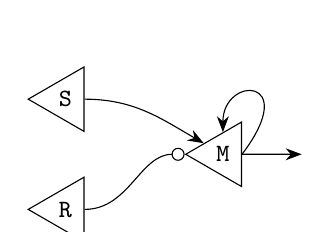
\begin{tikzpicture}
    [   neuron/.style=
        {   draw
        ,   regular polygon
        ,   regular polygon sides=3
        ,   shape border rotate=90
        ,   inner sep=2pt
        ,   node font=\small\ttfamily
        }
    ,   baseline=0pt
    ,   >={Stealth[scale=1.2]}
    ]
    \node[neuron] (S) at (0cm, 7mm) {S};
    \node[neuron] (R) at (0cm,-7mm) {R};
    \node[neuron] (M) at (2cm, 0cm) {M};
    \draw[->] (S) to[out=0,in=150] (M);
    \draw[-o] (R) to[out=0,in=180] (M);
    \draw[->] (M.east) .. controls (3cm,1cm) and (2cm,1cm) .. (M);
    \draw[->] (M.east) to (3cm,0cm);
\end{tikzpicture}
 & & 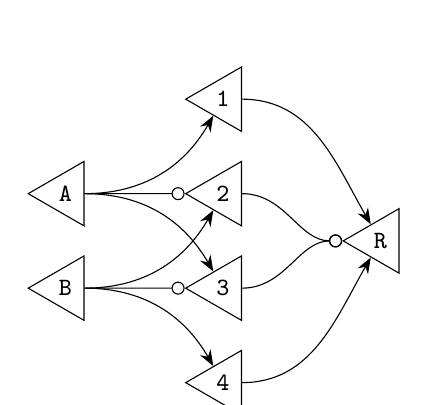
\begin{tikzpicture}
    [   neuron/.style=
        {   draw
        ,   regular polygon
        ,   regular polygon sides=3
        ,   shape border rotate=90
        ,   inner sep=2pt
        ,   node font=\small\ttfamily
        }
    ,   baseline=0pt
    ,   >={Stealth[scale=1.2]}
    ]
    \node[neuron] (A) at (-2cm, 6mm) {A};
    \node[neuron] (B) at (-2cm,-6mm) {B};
    \node[neuron] (Af) at (0cm, 18mm) {1};
    \node[neuron] (Ab) at (0cm,  6mm) {2};
    \node[neuron] (Ba) at (0cm, -6mm) {3};
    \node[neuron] (Bf) at (0cm,-18mm) {4};
    \node[neuron] (R) at (2cm,0cm) {R};
    \draw[->] (A) to[out=0,in=240] (Af);
    \draw[->] (B) to[out=0,in=120] (Bf);
    \draw[->] (Af) to[out=0,in=120] (R);
    \draw[->] (Bf) to[out=0,in=240] (R);
    \draw[->] (A) to[out=0,in=120] (Ba);
    \draw[->] (B) to[out=0,in=240] (Ab);
    \draw[-o] (A) to[out=0,in=180] (Ab);
    \draw[-o] (B) to[out=0,in=180] (Ba);
    \draw[-o] (Ab) to[out=0,in=180] (R.west);
    \draw[-o] (Ba) to[out=0,in=180] (R.west);
\end{tikzpicture}
\\
        $\displaystyle N_M(t+1) = (N_S(t) \vee N_M(t)) \wedge\neg N_R(t)$ &
        &
        $\displaystyle N_R(t+2) = N_A(t) \vee N_B(t)$\\
    \end{tabular}}{%
    Two common logic circuits using McCulloch's neurons
    where the arrows and circles indicate excitatory and inhibitory
    connections respectively.
}
While this model provided insight into the mechanisms by which neurons operate,
the structure was static, and incapable of learning.



McCulloch's work was later cited by psychologist \cite{Hebb:1949:Organization},
as important for understanding how logical operations are performed; but
proposed that the structure of biological neurons was dynamic, not static, and
that frequently repeated stimuli caused gradual development.
At the scale of neuron, it was theorised that if one neuron successfully
excited another, the connection between them would strengthen, hence
increasing the likelihood that the former would be able to excite the latter
again in the future.
His theory was supported by research conducted by himself and others that showed
that intelligence-test performance in mature patients was often unaffected by
brain operations that would have prevented development in younger patients,
which suggested that learnt stimuli are processed differently to unknown
stimuli.
This hypothesis became known as Hebbian learning.



Computer simulations applying this theory to a small network were done by
\cite{Farley:1954:Simulation}.
The actions of the network were compared to that of a servo system which must
counteract any displacements so as to maintain a steady position.
The network was trained using a set of input patterns, which were subject to
non-linear transformations.
Similar to the Hebbian theory, when the network produces the correct responses,
the active connections are strengthened.
Although the results were of little neurophysiological significance, they were
of great use for demonstrating computational simulations, which were
considerably slower at the time.



\subsection{Perceptrons}

The idea of the perceptron was originally conceived by
\cite{Rosenblatt:1958:Perceptron}, to represent a simplified model of
intelligent systems free from particularities of biological organisms, whilst
maintaining some of their fundamental properties.

The perceptron was built as a dedicated machine that consisted of a number of
photovoltaic cells, analogous to a retina, that feed into an ``association
area''.
This association area contains a number of cells that each calculate a weighted
sum of the receptor values and output a signal if it exceeds a threshold.
Expressed mathematically, the output of a given association cell is given by
\begin{align*}
    A_i &= \begin{cases}
        1, & \sum_j w_{i,j}x_j > \theta\\
        0, & \text{otherwise}
    \end{cases},
\end{align*}
where $x_j$ is the value from the $j^\text{th}$ photovoltaic cell, $w_{i,j}$
is the weight of the connection between association cell $i$ and photovoltaic
cell $j$, and $\theta$ is the activation threshold.
These value weights were implemented using variable resistance wires that the
perceptron could adjust automatically.
The outputs from the association area are then connected to response cells,
which operate in a similar fashion to the association cells.
The activation of these response cells are the outputs of the perceptron, and
indicated the classification of the input.

Similar to \cite{Farley:1954:Simulation}, the method by which the perceptron
adjusted it weights was also based on which cells were active, and whether the
correct output was produced; except that the perceptron was also able to
``penalise'' weights when an incorrect result was outputted.

This machine was initially trained to reliably identify three different shapes:
a square, a circle, and a triangle; and did so with a better than chance
probability.
When attempting to use the perceptron for more complicated tasks, such as
character recognition, it failed to produce better than chance results.



After a decade of unsuccessful real world application attempts, a book titled
``\citetitle{Minsky:1969:Perceptrons}'' by \cite{Minsky:1969:Perceptrons}, was
released.
The book provided a rigorous mathematical analysis of the model, the results
showed that single layered, simple linear perceptron networks could not
calculate XOR predicates.
A 2017 reissue of the book contained a foreword by L\'eon Bottou, who wrote
``Their rigorous work and brilliant technique does not make the perceptron look
very good...''



Following the book's release, perceptron research effectively halted for 15
years until the first successful uses of multilayer networks by
\cite{McClelland:1986:Parallel}, which also served as a departure from the
neuron outputs being boolean values.
The multilayered structure of this new model allowed it to calculate the XOR
predicates that the single layer perceptrons could not.

The output of the units within these networks were defined by
\begin{align*}
    \Rvec{a}(t+1) &= \Rvec{F}(\Rvec{a}(t),\Rvec{net}_1(t),\Rvec{net}_2(t),...),
\end{align*}
where $\Rvec{net}_i$ is the $i^\text{th}$ propagation rule applied to the
inputs, $\Rvec{F}$ is the activation function, and $\Rvec{a}(t)$ is the
activation of the units at time step $t$.
The model usually uses a simplified version which can be summarised as
\begin{align*}
    a_i &= F\left(\sum_j w_{i,j}o_j\right),
\end{align*}
where $o_j$ is the output of unit $j$.
Hebbian learning could be performed the network by using iterative methods,
the most simple of which was given by
\begin{align*}
    \Delta w_{i,j} &= \eta\,a_i o_j,
\end{align*}
where $\eta$ is the learning rate, which is a constant.

%\TODO{Subsection: Perceptrons}



\subsection{Backpropagation}

In order for a neural network to learn, it must undergo some form of
optimisation process.
For the perceptron, this process was one of positive and negative reinforcement.



In the field of control theory, an optimisation method known as gradient descent
was developed by \cite{Kelley:1960:Gradient}, in which a given function of the
system is either maximised or minimised.
This is achieved by taking partial derivatives of the function with respect to
each parameter, which gives an approximation of how the function value will
change as the parameter changes.
By evaluating the partial derivatives, multiplying them by a constant, and
adding them to their respective parameters, the parameter values can be updated.
Using these new parameter values, one can expect to improve the function value.
This can be written as
\begin{align*}
    w_i' &= w_i + \eta\Rpdiff{f}{w_i}(\Rvec{x}),
\end{align*}
where $f(\Rvec{x})$ is the function to be optimised, $w_i$ is a parameter of
$f$, $w_i'$ is the updated parameter, and $\eta$ is ascent/descent parameter.
Positive $\eta$ values will maximise the function value, where as negative
values will minimise it.
The magnitude of $\eta$ determines the rate at which the method will attempt
change the parameters: if the value is too large, the method will overshoot the
optimal values; if the value is too small, the method will be too slow to
converge.
This method is known as stochastic gradient descent.

When the method was applied to neural networks, researchers sometimes
encountered an issue now known as the vanishing gradient problem.
A computer program will typically calculate the gradient via repeat applications
of chain rule; if there are many small terms, the gradient will tend to zero,
and the learning rate of the network will be minimal.



One of the methods that overcame this problem was developed by
\cite{Schmidhuber:1992:Compression}, where each layer of the network was
pre-trained to predict the next input from previous inputs.
Once each layer had been pre-trained, the network was then fine tuned using
backpropagation.
The method also provided a way of calculating which inputs were least expected,
so that more training time could be devoted to learning them.

Since then, computational power has significantly increased, and the slow
convergence caused by the vanishing gradient problem is less significant.
Further more, backpropagation and a simple variant the model outlined by
\cite{McClelland:1986:Parallel}, have become the standard for neural networks.
Namely
\begin{align*}
    y_i &= \phi\left(b_i + \sum_j w_{i,j} x_j\right),
\end{align*}
where $x_j$ is the $j^\text{th}$ input, $w_{i,j}$ is the weight of connection
from $j$ to $i$, $b_i$ is the input bias of $i$, and $\phi$ is the activation
function.

%\TODO{Subsection: Backpropagation}



\section{Other Types of Artificial Neural Networks}

The preceding discussion has been focused on densely connected neural
networks, where each neuron in a layer is connected to every neuron in the
previous, but it is important to note, that many other neural network
architectures are often used together, and maybe more suitable under certain
contexts.

%\TODO{Section: Types of Neurons}



\subsection{Convolutional Neural Networks}
\label{subsec:history:conv}

Many of the neural networks that had been employed for image recognition, such
as the perceptron, suffered from two major issues:
\begin{enumerate}
    \item processing high resolution images required each neuron in the first
        layer to be connected to every input, which caused the number of
        connections to become too large to process; and,
    \item most networks could not correctly identify an input if it was shifted.
\end{enumerate}
Similar to how biology inspired neural networks, findings in neurophysiology
inspired the architectures that would overcome these issues.
\cite{Hubel:1959:Receptive}, discovered that certain cells within a cat's
visual cortex would only respond to stimuli from specific regions of the retina.
Another important observation was that neighboring cells had overlapping
response regions.

Later research by \cite{Hubel:1962:Receptive}, also distinguished two categories
of cells termed: ``simple'' and ``complex''.
Simple cells had distinct excitatory and inhibitory connections, where
firing was maximised by light slits at specific angles that passed through the
centre.
Complex cells could not be mapped out as trivial inhibitory/excitatory regions,
but were maximised by light slits at specific angles, regardless of position.



These findings inspired \cite{Fukushima:1980:Neocognitron}, to design the
neocognitron.
The neocognitron featured alternating layers of ``S-Planes'' and ``C-Planes'',
which were representations of the simple and complex cells respectively.
Each plane contains a number of feature maps, each unit within a feature map
is a function of a small region of the previous layer, a process now commonly
referred to as convolution.
S-Plane feature maps connect to all feature maps of the previous layer,
but C-Plane feature maps only connect to the corresponding feature map.
\rfig{\HIDE{
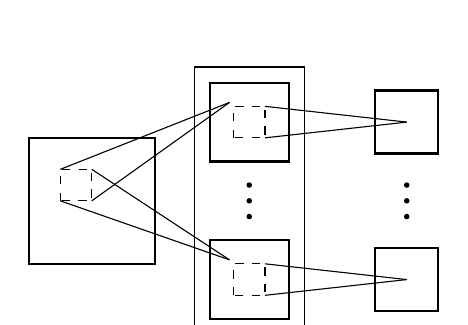
\begin{tikzpicture}
    \draw[thick] (-8mm,-8mm) rectangle (8mm,8mm);
    \draw[dashed] (-4mm, 0mm) rectangle (0mm,4mm);

    \draw[thick] (15mm,  5mm) rectangle ++(10mm,10mm);
    \foreach\y in {-2,0,2}
    {   \fill (20mm,1mm*\y) circle (1pt);
    }
    \draw[thick] (15mm,-15mm) rectangle ++(10mm,10mm);

    \draw (13mm,-17mm) rectangle (27mm,17mm);

    \draw (-4mm,4mm) -- (20mm-2.5mm, 10mm+2.5mm);
    \draw (20mm-2.5mm, 10mm+2.5mm) -- (0mm,0mm);
    \draw (0mm,4mm) -- (20mm-2.5mm,-10mm+2.5mm);
    \draw (20mm-2.5mm,-10mm+2.5mm) -- (-4mm,0mm);

    \draw[thick] (36mm, 6mm) rectangle ++(8mm,8mm);
    \foreach\y in {-2,0,2}
    {   \fill (40mm,1mm*\y) circle (1pt);
    }
    \draw[thick] (36mm,-14mm) rectangle (44mm,-6mm);

    \foreach\y in {-10,10}
    {   \draw[dashed] (18mm,1mm*\y-2mm) rectangle ++(4mm,4mm);
        \draw (22mm,1mm*\y+2mm) -- (40mm,1mm*\y);
        \draw (40mm,1mm*\y) -- (22mm,1mm*\y-2mm);
    }
\end{tikzpicture}
}
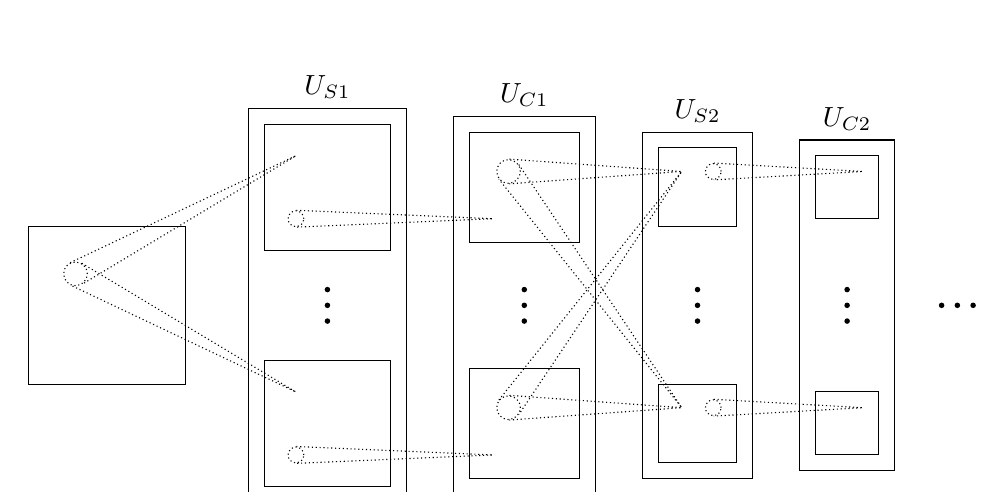
\begin{tikzpicture}
    [   kerline/.style =
        {   line join=round
        ,   densely dotted
        },
        kernel/.style =
        {   draw
        ,   circle
        ,   densely dotted
        }
    ]
    \newcommand{\kerlines}[2]{%
        \draw[kerline] (tangent cs:node=#1,point={(#2)},solution=1)
            -- (#2) -- (tangent cs:node=#1,point={(#2)},solution=2);
    }
    \newcommand{\kerdots}[1]{%
        \foreach\y in {-2,0,2}
        {   \fill (#1,1mm*\y) circle (1pt);
        }
    }

    %% planes
    % U0
    \node (U0) at ( 0mm,  0mm) [draw,rectangle,minimum size=20mm] {};
    % US1
    \node (US1G1) at (28mm,-15mm) [draw,rectangle,minimum size=16mm] {};
    \kerdots{28mm}
    \node (US1G2) at (28mm, 15mm) [draw,rectangle,minimum size=16mm] {};
    \draw (18mm,-25mm) rectangle (38mm,25mm);
    \node at (28mm,25mm) [above] {$U_{S1}$};
    % UC1
    \node (UC1G1) at (53mm,-15mm) [draw,rectangle,minimum size=14mm] {};
    \kerdots{53mm}
    \node (UC1G2)at (53mm, 15mm) [draw,rectangle,minimum size=14mm] {};
    \draw (44mm,-24mm) rectangle (62mm,24mm);
    \node at (53mm,24mm) [above] {$U_{C1}$};
    % US2
    \node (US2G1) at (75mm,-15mm) [draw,rectangle,minimum size=10mm] {};
    \kerdots{75mm}
    \node (US2G2) at (75mm, 15mm) [draw,rectangle,minimum size=10mm] {};
    \draw (68mm,-22mm) rectangle (82mm,22mm);
    \node at (75mm,22mm) [above] {$U_{S2}$};
    % UC2
    \node (UC2G1) at (94mm,-15mm) [draw,rectangle,minimum size=8mm] {};
    \kerdots{94mm}
    \node (UC2G2) at (94mm, 15mm) [draw,rectangle,minimum size=8mm] {};
    \draw (88mm,-21mm) rectangle (100mm,21mm);
    \node at (94mm,21mm) [above] {$U_{C2}$};

    %% kernels
    % U0 -> US1
    \coordinate (U0tUS1) at (-4mm,+4mm);
    \node[kernel] (U0K) at ($(U0)+(U0tUS1)$)
        [inner sep=0pt,minimum size=3mm] {};
    \coordinate (US1P1) at ($(US1G1)+(U0tUS1)$);
    \coordinate (US1P2) at ($(US1G2)+(U0tUS1)$);
    \kerlines{U0K}{US1P1}
    \kerlines{U0K}{US1P2}
    % US1 -> UC1
    \coordinate (US1tUC1) at (-4mm,-4mm);
    \node[kernel] (US1K1) at ($(US1G1)+(US1tUC1)$)
        [inner sep=0pt,minimum size=2mm] {};
    \node[kernel] (US1K2) at ($(US1G2)+(US1tUC1)$)
        [inner sep=0pt,minimum size=2mm] {};
    \coordinate (UC1P1) at ($(UC1G1)+(US1tUC1)$);
    \coordinate (UC1P2) at ($(UC1G2)+(US1tUC1)$);
    \kerlines{US1K1}{UC1P1}
    \kerlines{US1K2}{UC1P2}
    % UC1 -> US2
    \coordinate (UC1tUS2) at (-2mm,2mm);
    \node[kernel] (UC1K1) at ($(UC1G1)+(UC1tUS2)$)
        [inner sep=0pt,minimum size=3mm] {};
    \node[kernel] (UC1K2) at ($(UC1G2)+(UC1tUS2)$)
        [inner sep=0pt,minimum size=3mm] {};
    \coordinate (US2P1) at ($(US2G1)+(UC1tUS2)$);
    \coordinate (US2P2) at ($(US2G2)+(UC1tUS2)$);
    \kerlines{UC1K1}{US2P1}
    \kerlines{UC1K1}{US2P2}
    \kerlines{UC1K2}{US2P1}
    \kerlines{UC1K2}{US2P2}
    % US2 -> UC2
    \coordinate (US2tUC2) at (2mm,2mm);
    \node[kernel] (US2K1) at ($(US2G1)+(US2tUC2)$)
        [inner sep=0pt,minimum size=2mm] {};
    \node[kernel] (US2K2) at ($(US2G2)+(US2tUC2)$)
        [inner sep=0pt,minimum size=2mm] {};
    \coordinate (UC2P1) at ($(UC2G1)+(US2tUC2)$);
    \coordinate (UC2P2) at ($(UC2G2)+(US2tUC2)$);
    \kerlines{US2K1}{UC2P1}
    \kerlines{US2K2}{UC2P2}

    \foreach\x in {106,108,110}
    {   \fill (1mm*\x,0mm) circle (1pt);
    }
\end{tikzpicture}
}{%
    Representation of the neocognitron's connectivity.
}
Each layer of the network reduces the size of input image until the final layer
consists of single unit feature maps.
The network was originally trained to distinguish 5 digits, numbers 0 to 4,
using an unsupervised learning method, and was the first to reliably handle
shifted inputs.



\cite{Waibel:1989:Phoneme}, used concepts from the neocognitron to design the
time delay neural network, which was originally proposed for phoneme
recognition.
The networks were initially trained using backpropagation to detect and
distinguish between three acoustically similar phonemes (/b/, /d/, and /g/).
The model consisted of units similar to the neocognitron's S-Planes, where the
output of a unit is a function of a region from the previous layer.
The input for the model was a 2D spectrogram of an audio sample, with each
column representing a set of 16 spectral coefficients for a given time frame.

The first hidden layer contained columns of 8 units, each of which convolved the
spectral coefficients across 3 time frames, requiring a total of 384 weights.
Similarly, the second hidden layer contained columns of 3 units, each convolving
the previous layer across 5 time frames, requiring a total of 120 weights.
Finally, the output layer contains three units, each of which is a function of
the previous layer's corresponding row sum.
The most active unit is the phoneme present in the audio.

Once trained, the network was able to detect the correct phoneme, in real time,
under a variety of contexts, with an error of 1.5\%, a significant improvement
over the 6.3\% error from the most popular method at the time.



Similar techniques were used by \cite{LeCun:1989:Backpropagation}, to classify
handwritten digits.
A large number of 16 by 16 pixel images were used to train the network using
backpropagation.
The network consisted of two convolutional layers, and two dense layers.
Although the all of the units in a feature map shared the same weights, each
had a unique, adjustable bias.
Once trained, the network correctly classified 99.86\% of the training data, and
95\% of the test data.



This technique of combining convolutional and dense dense layers was also used
by \cite{Yamaguchi:1990:Neural}, for speech recognition.
Similar to \citeauthor{Waibel:1989:Phoneme}, the network takes a 2D spectrogram
as it's input and predicts which word was spoken.

The first layer, referred to as the event-net, convolves the input spectrogram
using a two layer subnetwork, which consists of a hidden partially connected
layer, and a fully connected single unit output layer.
Backpropagation is used to train each subnetwork of the event-net to only fire
when a word of the corresponding category is inputted.

The second layer, referred to as the time-alignment procedure, performs an
operation now known as max pooling, where each unit of the layer is the largest
value from the response region. If all the values are similar, use the one from
the middle of the search range; if all of the values are very low, the response
region size is increased

The third layer, referred to as the word-net, is another convolutional layer
using subnetwork, consisting of a fully connected layer, and a full connected
single unit output layer.
Backpropagation is used again in the same manner as in the event-net.

The forth layer, referred to as the super-net, is another convolutional
subnetwork that takes $N$ inputs and densely connects to $N+1$ outputs.
Each output corresponds to a word, except the last which denotes a rejected
result.

Finally, a decision algorithm compares the two highest outputs and rejects the
result if the difference does not exceed a preset threshold.



\subsection{Recurrent Neural Networks}

So far, the progression of time has been implemented as being another spacial
dimension.
Although this methodology proved effective for phoneme recognition tasks, it did
not work for other, more advanced temporal tasks.



\cite{Jordan:1986:Serial}, noted that representing time as a spacial dimension
required the network inputs to be stored in a buffer.
This buffer storage method was susceptible to a number of problems, including:
\begin{itemize}
    \item inability to account for input errors,
    \item lack of distinction between relative positions,
    \item difficulty with repeated actions, and
    \item difficulty processing different orderings of the same actions.
\end{itemize}
He proposed an alternative architecture, where the network takes the temporal
input in serial, whilst modifying its internal state.
This internal state is implemented by introducing cycles and delays into the
network.
Any network containing one or more cycles is described as being recurrent.

Such a network was initially trained to measure 8 phonetic features across time.
The input layer contained two groups of units:
input units, providing data from the current time frame;
and state units, providing compressed data from all previous time frames.
A hidden layer connects fully to all units from both groups in the input layer.
The output layer connects fully to the hidden layer.
The state units are connected to the output units and to themselves.
\rfig{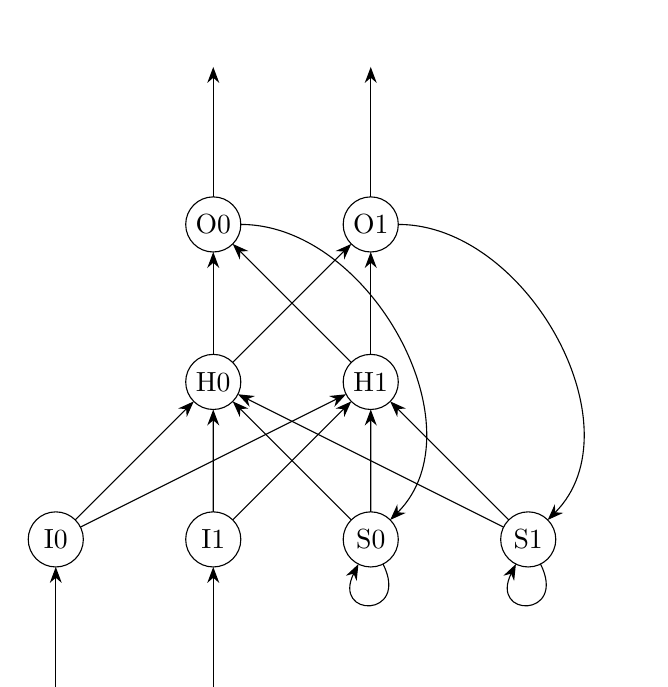
\begin{tikzpicture}
    [   > = {Stealth[scale=1.2]}
    ,   neuron/.style =
        {   draw
        ,   circle
        ,   inner sep = 0mm
        ,   outer sep = 0mm
        ,   minimum size = 7mm
        }
    ]
    \foreach\x in {0,1}
    {   \node[neuron] (I\x) at (\x*20mm-30mm, 0mm) {I\x};
        \node[neuron] (S\x) at (\x*20mm+10mm, 0mm) {S\x};
        \node[neuron] (H\x) at (\x*20mm-10mm,20mm) {H\x};
        \node[neuron] (O\x) at (\x*20mm-10mm,40mm) {O\x};
    }
    \foreach\x in {0,1}
    {   \foreach\y in {0,1}
        {   \draw[->] (I\x) to (H\y);
            \draw[->] (S\x) to (H\y);
            \draw[->] (H\x) to (O\y);
        }
        \draw[<-] (I\x) to ++(0mm,-20mm);
        \draw[->] (O\x) to ++(0mm, 20mm);
        \draw[->] (O\x) to[out=0,in=45] (S\x);
        \draw[->] (S\x) .. controls +( 5mm,-10mm) and +(-5mm,-10mm) .. (S\x);
    }

\end{tikzpicture}
}{%
    Example of Jordan's recurrent neural network.
}
During training, the network was exposed to one utterance at a time, and trained
to output the corresponding measures for each time frame.
For some combinations phonemes and features, any value is acceptable, these were
marked as ``don't-care'', and did not affect the error.
Due to the recurrent nature of the network, weight values were only updated
every 4 time steps.
The network learnt to process utterances and produce feature graphs that could
be used to identify the correct phonemes.



% \cite{Robinson:1987:Utility}
% based on control theory
% letter to word conversion
%   26 input, one for each letter
%   34 hidden
%   34 state
%    8 output, one for each word
%   learnt to output word at the start of the first letter of next word
% might not include



\cite{Elman:1990:Finding}, expanded Jordan's critiques of buffer-based
techniques by noting that there was no evidence of any biological equivalent.
He proposed that the state units should correspond to the hidden layer instead.
For each unit in the hidden layer, there is a corresponding state unit, which
holds the previous value of the hidden unit.
Units in the hidden layer is connected to the corresponding state unit, and
fully to the previous layer.
\rfig{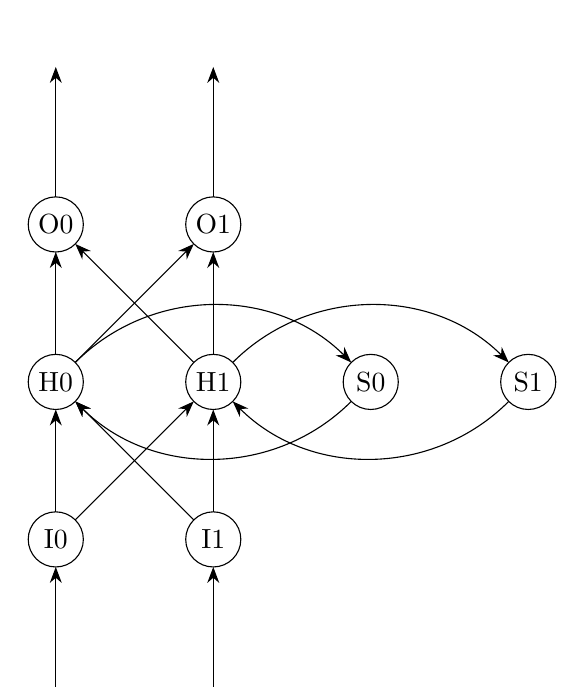
\begin{tikzpicture}
    [   > = {Stealth[scale=1.2]}
    ,   neuron/.style =
        {   draw
        ,   circle
        ,   inner sep = 0mm
        ,   outer sep = 0mm
        ,   minimum size = 7mm
        }
    ]
    \foreach\x in {0,1}
    {   \node[neuron] (I\x) at (20mm*\x, 0mm) {I\x};
        \node[neuron] (H\x) at (20mm*\x,20mm) {H\x};
        \node[neuron] (S\x) at (20mm*\x+40mm,20mm) {S\x};
        \node[neuron] (O\x) at (20mm*\x,40mm) {O\x};
    }
    \foreach\x in {0,1}
    {   \foreach\y in {0,1}
        {   \draw[->] (I\x) to (H\y);
            \draw[->] (H\x) to (O\y);
        }
        \draw[->] (H\x) to[out= 45,in=135] (S\x);
        \draw[->] (S\x) to[out=225,in=315] (H\x);
        \draw[<-] (I\x) to ++(0mm,-20mm);
        \draw[->] (O\x) to ++(0mm, 20mm);
    }

\end{tikzpicture}
}{%
    Example of Elman's recurrent neural network.
}
The network structure was initially used to predict sequential bit patterns.
In one such experiment, a number of random sentences were generated using a
small lexicon, and were presented to a network one character at a time without
breaks.
Each character was presented to the network as a 5-bit number, via 5 input
units.
The network processes this input using 20 hidden units each with a respective
state unit, and outputs a prediction of the next letter via 5 output units.

Once trained, the network struggled to predict the first letter of each randomly
selected word, but was able to accurately predict the letters that followed.



% \cite{Schmidhuber:1992:Learning}
% history compression
%   $o(t) = f(i(t),h(t))$, $h(t) = g(i(t-1),h(t-1))$
%   $o$ is output/prediction
%   $i$ is input
%   $h$ is hidden/internal state
%   $f$ and $g$ are functions
%\cite{Schmidhuber:1992:Learning} introduced the principle of history
%compression.
%A discrete time
%adaptive method for removing redundant information from sequences
%\begin{center}
%    \begin{tikzpicture}
    [   > = {Stealth[scale=1.2]}
    ,   func/.style=
        {   draw
        ,   circle
        ,   inner sep = 0mm
        ,   outer sep = 0mm
        ,   minimum size = 5mm
        }
    ,   bbox/.style=
        {   draw
        ,   rectangle
        ,   inner sep = 5mm
        }
    ]
    % box 0
    \node (B0) at (-30mm, 0mm) [bbox] {\phantom{\rule{30mm}{20mm}}};
    \node (F0) at (-30mm,-10mm) [func] {\small$f$};
    \node (G0) at (-15mm, 0mm) [func] {\small$g$};
    \node (I0) at (-30mm, 25mm) {$i(0)$};
    \node (O0) at (-30mm,-25mm) {$o(0)$};
    \draw[->] (B0.west) to[out=0,in=180] (F0);
    \draw[->] (B0.west) to (G0);
    \draw[->] (B0.north) to (F0);
    \draw[->] (B0.north) to[out=270,in=90] (G0);
    \draw[->] (I0) to (B0.north);
    \draw[->] (F0) to (O0);
    % box 1
    \node (B1) at (30mm, 0mm) [bbox] {\phantom{\rule{30mm}{20mm}}};
    \node (F1) at (30mm,-10mm) [func] {\small$f$};
    \node (G1) at (45mm, 0mm) [func] {\small$g$};
    \node (I1) at ( 30mm, 25mm) {$i(1)$};
    \node (O1) at ( 30mm,-25mm) {$o(1)$};
    \draw[->] (B1.west) to[out=0,in=180] (F1);
    \draw[->] (B1.west) to (G1);
    \draw[->] (B1.north) to (F1);
    \draw[->] (B1.north) to[out=270,in=90] (G1);
    \draw[->] (I1) to (B1.north);
    \draw[->] (F1) to (O1);
    % inter
    \node[above] (0mm,0mm) {h(1)};
    \node (H0) at (-70mm,0mm) {h(0)};
    \node (H2) at ( 70mm,0mm) {h(2)};
    \draw[->] (G0) to (B1.west);
    \draw[->] (H0) to (B0.west);
    \draw[->] (G1) to (H2);
\end{tikzpicture}

%    \captionof{figure}{Visualisation of history compression.}
%\end{center}



The recurrent neural networks previously described performed well for problems
with short time delays, but failed to perform tasks involving more than 10
discrete time steps.
The reason for this is the vanishing/exploding gradient problem.
Because errors backpropagate through the recurrent connections across multiple
time steps, the errors either tend towards zero or infinity.

A solution to this problem was proposed by \cite{Hochreiter:1997:Long}, where
the error term of the memory unit could be guaranteed to be a fixed constant.
This was achieved by using multiplicative gates to control the input and output
of the memory cell, resulting in a ``constant error carousel''.

Each cell took a weighted sum of the inputs and own previous state; and applied
a nonlinear function $g$ to obtain the net input signal, which connects to a
single, self-connected state unit.
A nonlinear function $h$ is applied to the value of the state unit to obtain
the output signal.
Gate units were controlled by taking a weighted sum of the layers inputs and
outputs, applying a nonlinear function, and multiplying by the relevant signal.
These gates prevented the network from perturbing its state, and prevents the
cell state from perturbing the reset of the network, allowing it to learn
long-lag-time tasks,
This new neural architecture was termed ``Long Short-Term Memory'' (LSTM).
% recurrent network architecture
% appropriate gradient-based learning algorithm
% variant of RTRL for learning



Although LSTM networks could learn long-lag-time tasks, they could not learn
certain, very long inputs that contain multiple sub-sequences.
This was because continual input streams would cause the cell state to grow
without bound, even in cases where the inputs suggest that the state should be
occasionally reset.
This problem was solved by \cite{Gers:1999:Learning}, by introducing a third
gate to the LSTM, which controlled the cell's internal recurrent connection.

It should be noted that an LSTM cell can ``learn to never forget'', hence
recovering the previous model.
% LSTM fails to learn to correctly process certain very long or continual time
% series that are not a priori segmented into appropriate training subsequences
% with clearly defined beginnings and ends
% continual input stream eventually may cause the internal values of the cells
% to grow without bound, even if the repetitive nature of the problem suggests
% they should be reset occasionally
% introduced forget gate
% formulation allows for the network to learn to never forget inputs, hence new
% model is an expansion of the previous and can solve any problem that the
% previous could



A further expansion of the model by \cite{Gers:2000:Recurrent}, added
``peephole'' connections between the internal state unit and the gates, allowing
the gates to access the state, even when the output gate was closed.
Additionally, the output function, $h$, was removed, as there was no empirical
evidence to suggest it was required.

These peephole connections allowed the model to perform count and timing tasks,
such as producing nonlinear, precisely timed spikes.
A full diagram is given in Figure \ref{INN:LSTM}

\newpage
\rfig{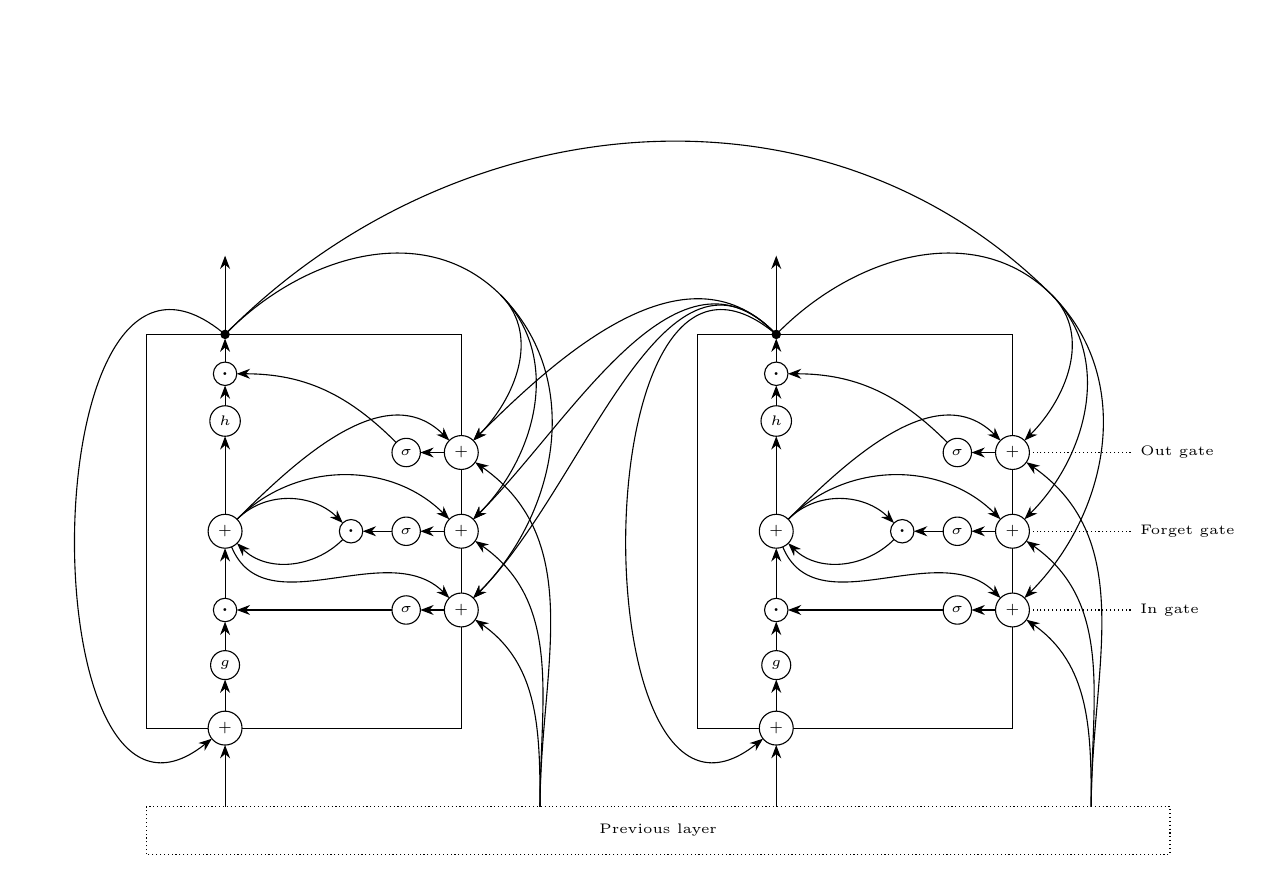
\begin{tikzpicture}
    [   > = {Stealth}
    ,   neuron/.style =
        {   draw
        ,   circle
        ,   fill = white
        ,   inner sep = 2pt
        ,   outer sep = 0mm
        }
    ,   route/.style =
        {   draw
        ,   circle
        ,   fill = black
        ,   inner sep = 0mm
        ,   outer sep = 0mm
        ,   minimum size = 3pt
        }
    ,   phant/.style =
        {   inner sep = 0mm
        ,   outer sep = 0mm
        ,   minimum size = 0mm
        }
    ]
    \foreach\n in {0,1}
    {   \pgfmathtruncatemacro{\x}{70*\n-35}
        \draw (1mm*\x-20mm,-25mm) rectangle (1mm*\x+20mm,25mm);
        \node[phant] (L\n) at (1mm*\x-25mm,30mm) {};
        \node[phant] (R\n) at (1mm*\x+25mm,30mm) {};

        \node[neuron] (I\n) at (1mm*\x-10mm,-25mm) {\tiny$+$};
        \node[neuron] (F\n) at (1mm*\x-10mm,-17mm) {\tiny$g$};
        \draw[->] (I\n) to (F\n);
        \draw[<-] (I\n) to ++(0mm,-10mm);

        \node[route] (O\n) at (1mm*\x-10mm,25mm) {};
        \node[neuron] (G\n) at (1mm*\x-10mm,14mm) {\tiny$h$};
        \node[neuron] (OM\n) at (1mm*\x-10mm,20mm) {.};
        \draw[->] (G\n) to (OM\n);
        \draw[->] (OM\n) to (O\n);
        \draw[->] (O\n) to ++(0mm,10mm);

        \node[neuron] (IG\n) at (1mm*\x+20mm,-10mm) {\tiny$+$};
        \node[neuron] (IF\n) at (1mm*\x+13mm,-10mm) {\tiny$\sigma$};
        \node[neuron] (IM\n) at (1mm*\x-10mm,-10mm) {.};
        \draw[->] (IG\n) to (IF\n);
        \draw[->] (F\n) to (IM\n);
        \draw[->] (IF\n) to (IM\n);

        \node[neuron] (FG\n) at (1mm*\x+20mm,0mm) {\tiny$+$};
        \node[neuron] (FF\n) at (1mm*\x+13mm,0mm) {\tiny$\sigma$};
        \draw[->] (FG\n) to (FF\n);

        \node[neuron] (OG\n) at (1mm*\x+20mm,10mm) {\tiny$+$};
        \node[neuron] (OF\n) at (1mm*\x+13mm,10mm) {\tiny$\sigma$};
        \draw[->] (OG\n) to (OF\n);
        \draw[->] (OF\n) to[out=135,in=0] (OM\n);

        \node[neuron] (M\n) at (1mm*\x-10mm,0mm) {\tiny$+$};
        \node[neuron] (MM\n) at (1mm*\x+6mm,0mm) {.};
        \draw[->] (FF\n) to (MM\n);
        \draw[->] (M\n) to[out=45,in=135] (MM\n);
        \draw[->] (MM\n) to[out=225,in=315] (M\n);
        \draw[->] (IM\n) to (M\n);
        \draw[->] (M\n) to (G\n);

        \draw[-] (O\n) to[out=45,in=135] (R\n);
        \draw[->] (R\n) to[out=315,in=45] (IG\n);
        \draw[->] (R\n) to[out=315,in=45] (FG\n);
        \draw[->] (R\n) to[out=315,in=45] (OG\n);

        \draw[->] (O\n) .. controls +(-25mm,20mm) and +(-25mm,-20mm)  .. (I\n);
        \draw[->] (1mm*\x+30mm,-35mm) to[out=90,in=325] (IG\n);
        \draw[->] (1mm*\x+30mm,-35mm) to[out=90,in=325] (FG\n);
        \draw[->] (1mm*\x+30mm,-35mm) to[out=90,in=325] (OG\n);
        %peep hole connectionss
        \draw[->] (M\n) to[out=-67.5,in=135] (IG\n);
        \draw[->] (M\n) to[out=45,in=135] (FG\n);
        \draw[->] (M\n) to[out=45,in=135] (OG\n);
    }
    %\draw[-] (O1) to[out=135,in=45] (L1);
    %\draw[->] (L1) to[out=225,in=45] (IG0);
    %\draw[->] (L1) to[out=225,in=45] (FG0);
    %\draw[->] (L1) to[out=225,in=45] (OG0);
    \draw[-] (O0) to[out=45,in=135] (R1);
    \draw[->] (O1) to[out=135,in=45] (IG0);
    \draw[->] (O1) to[out=135,in=45] (FG0);
    \draw[->] (O1) to[out=135,in=45] (OG0);
    \node[anchor=west] (IL) at ($(IG1)+(15mm,0mm)$) {\tiny In gate};
    \node[anchor=west] (FL) at ($(FG1)+(15mm,0mm)$) {\tiny Forget gate};
    \node[anchor=west] (OL) at ($(OG1)+(15mm,0mm)$) {\tiny Out gate};
    \draw[densely dotted] (IL) to (IG1);
    \draw[densely dotted] (FL) to (FG1);
    \draw[densely dotted] (OL) to (OG1);
    \draw[densely dotted] (-55mm,-41mm) rectangle (75mm,-35mm);
    \node at (10mm,-38mm) {\tiny Previous layer};
\end{tikzpicture}
}{%
    Visualisation of two LSTM units, where $\sigma$,
    $g$, and $h$ are function units;
    $+$ is a weighted summation unit; and $\cdot$ is multiply unit.
}\label{INN:LSTM}
% during learning no error signals are propagated back from gates
% via peephole connections




\chapter{Introduction to Python}

Python is a general-purpose programming language designed by Guido van Rossum,
with an emphasis on readability and reusability \citep{vanRossum:1996:Foreword}.
It comes with an extensive standard library and is one of the most popular
programming languages.

There are multiple options for interacting with Python, these include:
\begin{itemize}
    \item typing commands into an interpreter,
    \item writing files and running them with an interpreter,
    \item using an online service such as Google Colab.
\end{itemize}
A small snippet of trivial python code is given below to display the syntax.
{\singlespacing
\inputminted[
    frame=lines,
    framesep=2mm,
    mathescape,
    linenos
    ]{python}{Sample.py}
}

\section{Neural Networks in Python}

Before using any neural network packages, a few small examples networks were
produced in python.
The \texttt{numpy} package was used to perform matrix operations,
and the \texttt{matplotlib.pyplot} package was used for plotting,
as these features were non-trivial.
For some examples, the \texttt{keras} module from the \texttt{tensorflow}
package was also used to access specific datasets, but their broader purpose
will be explored in the next section.

\subsection{Single Layer Boston Housing Data}

The first example network consisted of 3 input neurons connected to a
single output neuron, which is given by the equation
\begin{align*}
    y &= \tanh\left(b + \sum_{i=1}^{3} w_ix_i\right).
\end{align*}
The bias term was implemented by adding a forth input node with a constant value
of one, giving
\begin{align*}
    y &= \tanh\left(\mathbf{w}\cdot\mathbf{x}\right),
\end{align*}
where $w_4 = b$, and $x_4 = 1$.

The network was trained using the Boston housing dataset from \texttt{keras},
which provided a number of attributes about houses from late 1970's Boston
suburbs.
The network took in normalised data from three of these attributes (number of
rooms, highway accessibility index, percentage of lower status population), and
used them to predict the value of the house.

Training was performed using backpropagation, defined by the equation
\begin{align*}
    \Delta w_i &= \eta\Rpdiff{e}{w_i},\\
    d &= y - y_t,\\
    e &= \frac{1}{2}d^2,
\end{align*}
where $e$ is the network error, $y$ is the network prediction, and $y_t$ is the
target value.
By definition,
\begin{align*}
    y &= \tanh(\text{net}),\\
    \text{net} &= \sum w_ix_i.
\end{align*}
By chain rule,
\begin{align*}
    \Rpdiff{e}{w_i} &=
    \Rpdiff{e}{y} \cdot \Rpdiff{y}{\text{net}} \cdot \Rpdiff{\text{net}}{w_i}.\\
    %
    \Rpdiff{net}{w_i} &= x_i,\\
    \Rpdiff{y}{net} &= 1 - \tanh^2(net) = 1 - y^2,\\
    \Rpdiff{e}{y} &= \frac{1}{2}\Rpdiff{(y - y_t)^2}{y} = y - y_t = d,\\
    %
    \therefore\Rpdiff{e}{w_i} &=
    x_i \cdot (1 - y^2) \cdot d.
\end{align*}
$\Delta w_i$ can be written in vector notation, giving
\begin{align*}
    \Delta \mathbf{w} &= \eta\cdot\mathbf{x}\cdot (1-y^2)\cdot d.
\end{align*}
Weights were updated after each sample using
\begin{align*}
    \mathbf{w}' &= \mathbf{w} - \Delta\mathbf{w},
\end{align*}
where $\mathbf{w}'$ is the new set of weights.

The network was initialised using random weights, and was trained using the full
dataset.
\rfig{\begin{tikzpicture}
    \begin{axis}
        [   width = 0.8\textwidth
        ,   xtick = {0,1000,2000,3000,4000,5000}
        ,   legend pos = south west
        ,   xlabel = {Iteration}
        ,   ylabel = {Value}
        ]
        \addplot [color = Rblue]   table [col sep = comma]
        {../Code/BostonHousing/DataPythonSingleW0.csv};
        \addplot [color = Rorange] table [col sep = comma]
        {../Code/BostonHousing/DataPythonSingleW1.csv};
        \addplot [color = Rgreen]  table [col sep = comma]
        {../Code/BostonHousing/DataPythonSingleW2.csv};
        \addplot [color = Rred]    table [col sep = comma]
        {../Code/BostonHousing/DataPythonSingleW3.csv};
        \legend{$w_0$,$w_1$,$w_2$,$w_3$}

        \addplot
        [   opacity = 0.2
        ,   sharp plot
        ,   update limits = false
        ]   coordinates {(0,-1) (0,1)};
        \pgfplotsinvokeforeach{1,...,10}%
        {   \addplot
            [   opacity = 0.2
            ,   sharp plot
            ,   update limits = false
            ]   coordinates {(506*#1,-1) (506*#1,1)}
            node [anchor = south, rotate = 90] at (506*#1,0.05) {\tiny epoch = #1};
        }
    \end{axis}
\end{tikzpicture}
}{%
    Graph of network weights against iteration number.
}
After 10 epochs, the mean square error had reduced from 0.1637 to 0.0507.
Note that the weight value lines appear to be jagged, this was a side effect of
updating the value after each individual presentation; a problem which can be
mitigated by batching $\Delta\mathbf{w}$ terms from multiple presentations.



\subsection{Multilayer Boston Housing Data}

The same task was repeated using the full set of attributes.
To accommodate this, a larger network with 13 input neurons, 1 output neuron,
and $n$ hidden neurons; which was expressed by the equation
\begin{align*}
    h_i &= \tanh\left(b_i + \sum_{j=0}^{13} w_{i,j}x_j\right),\\
    y &= b + \sum_{i=1}^{n} w_i h_i.
\end{align*}
Similar to the single layer example, a constant neuron was added to the input
and hidden layer to implement the bias, giving
\begin{align*}
    \mathbf{h} &= \tanh(W\mathbf{x}),\\
    \mathbf{h}' &= \begin{pmatrix} \mathbf{h} \\ 1 \end{pmatrix},\\
    y &= \mathbf{w}\cdot\mathbf{h}',
\end{align*}
where $\tanh$ acts component-wise on the input.

All of the inputs were batched together into a single matrix $X$, where each
column was a data point, giving
\begin{align*}
    \Phi &= \tanh(W\cdot X),\\
    \Psi &= \begin{pmatrix} \Phi \\ \mathbf{1} \end{pmatrix},\\
    \mathbf{y} &= \mathbf{w}\cdot\Psi,
\end{align*}
where $\mathbf{y}$ is a row vector of results.
The error gradients for the output neurons were given by
\begin{align*}
    \mathbf{d} &= \mathbf{y} - \mathbf{y}_t,\\
    e &= \frac{1}{2}\left|\mathbf{d}\right|^2,\\
    \mathbf{g}_O &= \Rpdiff{e}{\mathbf{w}} = \mathbf{d}\cdot\Psi^T;
\end{align*}
and for the hidden neurons by
\begin{align*}
    D &= \hat{\mathbf{w}}^T\cdot\mathbf{d},\\
    G_H &= ((1 - \Phi\odot\Phi)\odot D) \cdot X^T,
\end{align*}
where $\odot$ is the component-wise product, and $\hat{\mathbf{w}}$ is the
weight vector without the bias term.
Note that $\hat{\mathbf{w}}^T$ and $\mathbf{e}$ are column and row vectors
respectively, and that their product is a matrix.
See Appendix \ref{app:BHMDeriv} for full derivation.
\rfig{\begin{tikzpicture}
    \begin{axis}
        [   width = 0.8\textwidth
        ,   xtick = {0,100,200,300,400,500}
        ,   legend pos = north east
        ,   xlabel = {Epoch}
        ,   ylabel = {Loss}
        ]
        \addplot [color = Rblue]   table [col sep = comma]
        {../Code/BostonHousing/DataPythonMulti1.csv};
        \addplot [color = Rorange] table [col sep = comma]
        {../Code/BostonHousing/DataPythonMulti2.csv};
        \addplot [color = Rgreen]  table [col sep = comma]
        {../Code/BostonHousing/DataPythonMulti3.csv};
        \legend{Hidden = 1,Hidden = 2,Hidden = 3}
    \end{axis}
\end{tikzpicture}
}{%
    Graph of network error against iteration number for
    various numbers of hidden neurons, using the Boston housing data.
}
The network was trained multiple times with varying numbers of hidden neurons.
The same random seed value was used for all trials.
In each case, the network successfully reduced it's error to roughly the same
level:
for 1 neuron, from 0.1670 to 0.0380;
for 2 neurons, from 0.1799 to 0.0390; and
for 3 neurons, from 0.1757 to 0.0396.
The difference between the results was negligible, which suggested that one
hidden neuron was sufficient for learning the data.

When compared with the single layer network from the previous section, the
single neuron, multilayer network performed better (0.0507 vs 0.0380) for two
reasons:
\begin{enumerate}
    \item it had access to all 13 attributes, instead of the 3 attributes that
        had been manually selected; and
    \item the additional layer enabled it to apply a linear transformation to
        the activation.
\end{enumerate}
Additionally, the use of batched inputs resulted in a smoother descent, as the
total gradient is descended; instead of multiple, often opposing gradients.



\subsection{Logical XOR}

Using the same, multilayer network architecture, a network was trained to
perform the logical exclusive-or (XOR) operation.
The input matrix $X$ contained all four combinations of binary inputs, and the
target outputs in $\mathbf{y}_t$.
\begin{align*}
    X &= \begin{pmatrix}
        0 & 1 & 0 & 1 \\
        0 & 0 & 1 & 1 \\
        1 & 1 & 1 & 1
    \end{pmatrix},\\
    \mathbf{y}_t &= \begin{pmatrix}
        0 & 1 & 1 & 0
    \end{pmatrix}.
\end{align*}
Given that the problem is mathematically well defined, a successfully trained
network should reduce the error to near zero.
Training the network for varying numbers of hidden neurons gave the following
results.
\rfig{\begin{tikzpicture}
    \begin{axis}
        [   width = 0.8\textwidth
        ,   xtick = {0,50,100,150,200,250,300}
        ,   legend pos = north east
        ,   xlabel = {Epoch}
        ,   ylabel = {Loss}
        ]
        \addplot [color = Rblue]   table [col sep = comma]
        {../Code/XOR/DataPython1.csv};
        \addplot [color = Rorange] table [col sep = comma]
        {../Code/XOR/DataPython2.csv};
        \addplot [color = Rgreen]  table [col sep = comma]
        {../Code/XOR/DataPython3.csv};
        \legend{Hidden = 1,Hidden = 2,Hidden = 3}
    \end{axis}
\end{tikzpicture}
}{%
    Graph of network error against iteration number for
    various numbers of hidden neurons, using the XOR data.
}
The final mean square errors for one, two, and three hidden neurons were 0.1713,
$2.04\times10^{-5}$, and $9.65\times10^{-6}$ respectively.
These results showed that a single, nonlinear neuron is not sufficient for
learning the XOR problem, as proven by \cite{Minsky:1969:Perceptrons}, and is
only capable of solving three of the four inputs at a time.
Two nonlinear neurons is sufficient for solving the problem.

It is important to note that the learning rates were much more susceptible to
the initial weights than that of the Boston housing data.
Under certain initial conditions, the network displayed long periods of
negligible change before significant learning occurred, the longest of which
that had been observed lasted over 800 iterations.
Error spiking was observed across the majority of initial conditions for both
two and three hidden neurons.



\section{Using TensorFlow and Keras}

Creating efficient neural networks by hand was difficult, repetitive, and prone
to mistakes; and making simple modifications, such as changing the activation
function, could prove tricky for larger networks.
Thankfully, python packages that automate large portions of the process are
available, namely TensorFlow.

Once installed, TensorFlow can be imported into python.
TensorFlow contains a module called Keras, which provides a number of objects
and constructors that make the process much simpler.
The XOR network, for instance, can be constructed with a few lines of code.
\begin{minted}[
    frame=lines,
    framesep=2mm,
    mathescape,
    linenos
    ]{python}
import tensorflow as tf
layers = tf.keras.layers
# Create a model
model = tf.keras.models.Sequential()
# Add a dense hidden layer with the built in $\tanh$ activation function
model.add(layers.Dense(3, input_dim=2, activation='tanh')
# Add the output layer with linear activation
model.add(layers.Dense(1))
# Finalise the model and specify the loss function
model.compile(loss='mean_squared_error')
\end{minted}
TensorFlow provides multiple ways of constructing models, and a wide variety of
options to configure layers, models, and optimisers, as well as custom
definitions.

Once constructed, the model can be trained using the \texttt{fit} method, which
provides a history of network properties from each epoch; and used to predict
inputs using the \texttt{predict} method.
Models can be saved to a file using the \texttt{save} method, which includes the
network structure and weights, and loaded using
\texttt{tensorflow.keras.models.load\_model}.

TensorFlow also supports multithreading and GPU acceleration, making it
especially suitable for large networks and training sets.



\subsection{Optimisers and the Boston Housing Data}

The Boston housing example was repeated using TensorFlow, with two hidden
layers, each with five neurons using the $\tanh$ activation function, and a
linear output layer, to see if adding additional layers and neurons would
improve the results.
The data was also split into two groups, training and validation, the latter of
which was not used for training the network.
For a well-fitting network, the loss values for both groups should be similar,
and the ratio between them provided a rough measure of over-fitting.
\rfig{\begin{tikzpicture}
    \begin{axis}
        [   width = 0.8\textwidth
        ,   xtick = {0,500,1000,1500,2000}
        ,   ymin = 0
        ,   legend pos = north east
        ,   xlabel = {Epoch}
        ,   ylabel = {Loss}
        ]
        \addplot [color = Rblue]   table [col sep = comma]
        {../Code/BostonHousing/DataTensorSGDLoss.csv};
        \addplot [color = Rorange] table [col sep = comma]
        {../Code/BostonHousing/DataTensorSGDVali.csv};
        \legend{Training,Validation}
    \end{axis}
\end{tikzpicture}
}{%
    Graph of training and validation loss against iteration number for the
    Boston housing data using SGD.
}
%\newpage
The network was trained over 2000 epochs using the stochastic gradient descent
optimiser, obtaining an final training loss of 0.0421, and validation loss of
0.0396.
The ratio between the loss values is $\sim0.94$, this value is close to 1,
suggesting that the network was not over-fitting.

The network was trained again using the ``Adam'' optimiser
\citep{Kingma:2014:Adam}, which uses estimations of both first and second-order
moments, and consistently outperforms the stochastic gradient descent method.

With the Adam optimiser, the final training and validation loss values were
0.0147 and 0.0443 respectively.
Although the loss value is smaller than with stochastic gradient descent, the
loss ratio was $\sim3.01$, which suggests that the network was over-fitting.
This was further evidenced the loss graph, which show that beyond a certain
point, the training loss and validation loss diverge, with the validation loss
increasing.
As such, the network is expected to be less generalised.
\rfig{\begin{tikzpicture}
    \begin{axis}
        [   width = 0.8\textwidth
        ,   xtick = {0,500,1000,1500,2000}
        ,   ymin = 0
        ,   legend pos = north east
        ,   xlabel = {Epoch}
        ,   ylabel = {Loss}
        ]
        \addplot [color = Rblue]   table [col sep = comma]
        {../Code/BostonHousing/DataTensorAdamLoss.csv};
        \addplot [color = Rorange] table [col sep = comma]
        {../Code/BostonHousing/DataTensorAdamVali.csv};
        \legend{Training,Validation}
    \end{axis}
\end{tikzpicture}
}{%
    Graph of training and validation loss against iteration number for the
    Boston housing data using Adam.
}
When comparing the two optimisers, Adam trains the network significantly faster
than SGD.
Given a sufficient number of epochs, stochastic gradient descent will over-fit
the data, just as it did with Adam.
\newpage\noindent
TensorFlow provided eight optimisers at the time writing:
\begin{enumerate}

    \item\textsc{SGD}, stochastic gradient descent, uses a first-order error
        approximation;

    \item\textsc{Adam}, uses a first and second-order error approximation
        \citep{Kingma:2014:Adam};

    \item\textsc{AdaMax}, Adam variant based on the infinity norm
        \citep{Kingma:2014:Adam};

    \item\textsc{AdaGrad}, uses parameter-specific learning rates based on
        update frequency \citep{Duchi:2011:Adagrad};

    \item\textsc{AdaDelta}, stochastic gradient descent with adaptive learning
        rates \citep{Zeiler:2012:Adadelta};

    \item\textsc{RMSProp}, uses a root-mean-squared approach to adjust the
        learning rate \citep{Hinton:2014:RMSProp}.

    \item\textsc{NAdam}, Adam variant using Nesterov momentum
        \citep{Dozat:2016:NAdam}.

    \item\textsc{FTRL}, follow the regularized leader, online learning
        algorithm \citep{McMahan:2013:FTRL}.

\end{enumerate}
The optimal choice of optimiser varies with the network and data set size.
Adaptive rate optimisers, such as Adagrad, perform best with sparse input data;
but Adam, Adamax, NAdam, and RMSProp are typically the best options.
See next page for figure.

The overhead of each optimiser is minimal, and is unlikely to affect the time
taken to train the network.

The choice of optimiser is provided when compiling the model, via the
\texttt{optimizer} argument.
If no optimiser if provided, the default option, which was RMSProp, will be
used.
If a string is provided, TensorFlow will use the corresponding optimiser with
default parameters.
If an optimiser instance is provided, that instance will be used.

One may also define their own optimiser class.

\rfig{\begin{tikzpicture}
    \begin{axis}
        [   width = 0.8\textwidth
        ,   xtick = {0,500,1000,1500,2000}
        ,   ymin = 0
        ,   legend pos = north east
        ,   xlabel = {Epoch}
        ,   ylabel = {Loss}
        ]
        \addplot [color = Rblue]   table [col sep = comma]
        {../Code/BostonHousing/DataTensorVarySGDLoss.csv};
        \addplot [color = Rorange] table [col sep = comma]
        {../Code/BostonHousing/DataTensorVaryAdamLoss.csv};
        \addplot [color = Rgreen]  table [col sep = comma]
        {../Code/BostonHousing/DataTensorVaryAdagradLoss.csv};
        \addplot [color = Rred]    table [col sep = comma]
        {../Code/BostonHousing/DataTensorVaryAdadeltaLoss.csv};
        \addplot [color = Rpurple] table [col sep = comma]
        {../Code/BostonHousing/DataTensorVaryAdamaxLoss.csv};
        \addplot [color = Rpink]   table [col sep = comma]
        {../Code/BostonHousing/DataTensorVaryFTRLLoss.csv};
        \addplot [color = Raqua]   table [col sep = comma]
        {../Code/BostonHousing/DataTensorVaryNAdamLoss.csv};
        \addplot [color = Rocean]  table [col sep = comma]
        {../Code/BostonHousing/DataTensorVaryRMSpropLoss.csv};
        \legend{SGD,Adam,AdaGrad,AdaDelta,AdaMax,FTRL,NAdam,RMSProp}
    \end{axis}
\end{tikzpicture}
}{%
    Graph of training loss against time for the Boston housing data using
    various optimisers.
}

%2000 epochs

%SGD [5,5]
%initial loss 0.228166446089744570
%  final loss 0.042430859059095380
%initial vali 0.214338675141334530
%  final vali 0.046398963779211044
% vali / loss 1.093519311

%SGD [3,3]
%initial loss 0.285416126251220700
%  final loss 0.033157549798488620
%initial vali 0.329692572355270400
%  final vali 0.045487113296985626
% vali / loss

%SGD [3]
%initial loss 0.494845181703567500
%  final loss 0.041440241038799286
%initial vali 0.568243682384491000
%  final vali 0.048694450408220290

%Adams [5,5]
%initial loss 0.425099462270736700
%  final loss 0.014745806343853474
%initial vali 0.409027785062789900
%  final vali 0.044336102902889250

\subsection{Activation Functions and Character Recognition}

So far, only $\tanh$ and linear activation functions have been considered.
TensorFlow provides a total of eleven activation functions:
\begin{itemize}
    \item\texttt{linear}, no activation function applied,
        \begin{align*}
            \phi(x) &= x,
        \end{align*}

    \item\texttt{relu}, rectified linear unit,
        \begin{align*}
            \phi(x) &= \begin{cases}
                m, & x > m\\
                \alpha x, & x < 0\\
                x, & \text{otherwise}
            \end{cases},
        \end{align*}
        where $\alpha = 0$ and $m = \infty$ by default;

    \item\texttt{exponential},
        \begin{align*}
            \phi(x) &= e^x;
        \end{align*}

    \item\texttt{elu}, exponential linear unit,
        \begin{align*}
            \phi(x) &= \begin{cases}
                \alpha (e^x - 1) & x < 0\\
                x, & \text{otherwise}
            \end{cases},
        \end{align*}
        where $\alpha = 1$ by default;

    \item\texttt{selu}, special case of elu with an additional scaling factor
        and fixed parameters;

    \item\texttt{sigmoid},
        \begin{align*}
            \phi(x) &= \frac{1}{1 + e^{-x}};
        \end{align*}

    \item\texttt{hard\_sigmoid}, approximation of sigmoid using three linear
        segments,
        \begin{align*}
            \phi(x) &= \begin{cases}
                0, & x < -2.5\\
                1, & x > 2.5\\
                0.2x+0.5 & \text{otherwise}
            \end{cases};
        \end{align*}

    \item\texttt{tanh},
        \begin{align*}
            \phi(x) &= \frac{e^x - e^{-x}}{e^x + e^{-x}};
        \end{align*}

    \item\texttt{softsign}, smoothed sign function,
        \begin{align*}
            \phi(x) &= \frac{x}{|x| + 1};
        \end{align*}

    \item\texttt{softplus}, smoothed $\max(x,0)$ function,
        \begin{align*}
            \phi(x) &= \ln(e^x+1);
        \end{align*}

    \item\texttt{softmax}, normalised exponentials,
        \begin{align*}
            y_i &= \frac{e^{x_i}}{\sum_j e^{x_j}},
        \end{align*}
        where $x_i$ is the net value into softmax neuron $i$.
\end{itemize}

Categorisation task
Softmax: normalised exponentials

\rfig{\begin{tikzpicture}
    \loaddata{../Code/CharacterRecognition/FigrFlat.txt}
    \foreach\posx/\posy/\pred/\cert/\actu in \loadeddata
    {   \pgfmathtruncatemacro{\indx}{5*\posy+\posx}
        \node[draw] (N\indx) at (3*\posx,-3.8*\posy)
        {\includegraphics[width=1.5cm]{CRResults/img\indx}};
        \node (P\indx) at (N\indx.north) [anchor=south]
        {\scriptsize Predicted: \pred};
        \node (A\indx) at (P\indx.north) [anchor=south,outer sep=0,inner sep=0]
        {\scriptsize Was: \actu};
        \node (S\indx) at (N\indx.south) [anchor=north]
        {\scriptsize \ifnum \actu=\pred
                Correct
            \else
                \underline{\textbf{Incorrect}}
            \fi};
        \node (C\indx) at (S\indx.south) [anchor=north,outer sep=0,inner sep=0]
        {\scriptsize Certainty: \cert};
    }
\end{tikzpicture}
}{%
    Hand written numbers from the MNIST validation set, the network prediction,
    and the certainty of the network.
}
%500 epochs
%initial loss: 2.36568117141723630
%  final loss: 0.06899717450141907
%initial vali: 2.19691061973571780
%  final loss: 0.10314085334539413
%  training size:   60000
%validation size:   10000
%  training errors: 4223
%validation errors: 1247
%  training %err:   7.038333333333333
%validation %err:   12.47

%Convol: 50 epochs, batch=600
%initial loss: 0.574465834945440300
%initial vali: 0.247798308357596400
%final loss:   0.010112296480219812
%final loss:   0.058920445458497850
%training size:     60000
%training errors:   482
%training %err:     0.8033333333333333
%validation size:   10000
%validation errors: 493
%validation %err:   4.93

%own theory of composition
% functions f and g are compositionally similar if:
%  for small n:
%   \sum_{i=1}^{n} A_if(a_ix+b_i) + B = g(x)
%own theory of versatility
% function f is versatile if:
%  \sum_{i}^{\infty} A_if(a_ix+b_i) \approx \delta(\alpha)
% theory:
%  all discontinuous functions are versatile
%desirable properties of activation functions
% no vanishing/zero-gradient areas
% versatile
%  either discontinuous
%  or bounded

\subsection{Linear Regression}

\rfig{\begin{tikzpicture}
    \pgfplotsset{
        % define the layers you need.
        % (Don't forget to add `main' somewhere in that list!!)
        layers/my layer set/.define layer set =
        {   bottom
        ,   main
        ,   top
        }{
            % you could state styles here which should be moved to
            % corresponding layers, but that is not necessary here.
            % That is why wo don't state anything here
        },
        % activate the newly created layer set
    }
    \begin{axis}
        [   width = 0.8\textwidth
        ,   legend pos = north west
        ,   xmin = -0.1
        ,   ymin = -0.1
        ,   xmax =  1.1
        ,   ymax =  1.1
        ,   xtick = {0,0.2,0.4,0.6,0.8,1}
        ,   ytick = {0,0.2,0.4,0.6,0.8,1}
        ,   xlabel = {$x$}
        ,   ylabel = {$y$}
        ,   set layers = my layer set
        ]
        \addplot [on layer = bottom, color = Rblue, only marks, mark size = 1pt]
        table [col sep = comma]
        {../Code/Regression/DataLinearPoints.csv};
        \addplot [on layer = top, color = Rorange]
        table [col sep = comma]
        {../Code/Regression/DataLinearPrediction.csv};
        \legend{Data,Prediction}
    \end{axis}
\end{tikzpicture}
}{%
    Graph showing the data points and network's corresponding line of best fit.
}
%initial loss 0.62278741598129270000
%  final loss 0.00022495193115901202


\chapter{Reinforcement Learning}

The neural network structures previously discussed for the Boston Housing data
are essentially curve fitting models, with continuous inputs and output.
The character recognition networks for the MNIST dataset can also be though of
as an abstract curve fitting model with multiple outputs, where the result is
a probability value.

In both cases, training is performed on a set of inputs with known target
outputs.

Not all problems can be constructed in this manner as some problems require
discrete actions to be taken.
Similarly, problems may contain reward systems.
Such systems may have delayed rewards, were one action provides an immediate
reward, but prevents reaching a state of higher reward.

Consider the ``Chain'' problem from \cite{Strens:2000:ABF}:
\rfig{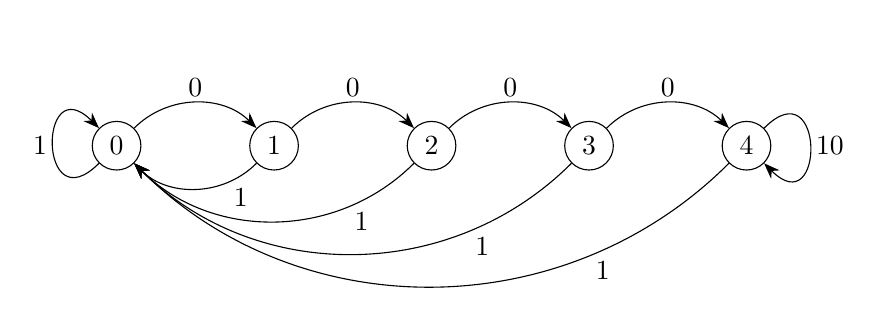
\begin{tikzpicture}
    [   state/.style=
        {   draw
        ,   circle
        }
    ,   baseline=0pt
    ,   >={Stealth[scale=1.2]}
    ]
    \foreach\n in {0,...,4}
    {   \node[state] (N\n) at (2cm*\n, 0mm) {$\n$};
    }
    \foreach\np in {1,...,4}
    {   \pgfmathtruncatemacro{\nm}{\np-1}
        \draw[->]
        (N\np)
            to [out=225,in=315]
            node [near start, anchor = north west, inner sep = 2pt] {1}
        (N0);
        \draw[->]
        (N\nm)
            to [out=45,in=135]
            node [anchor = south, inner sep = 2pt] {0}
        (N\np);
    }
    \draw[->]
    (N0)
        .. controls ++(-1cm,-1cm) and ++(-1cm,1cm) ..
        node [anchor = east, inner sep = 2pt] {1}
    (N0);
    \draw[->]
    (N4)
        .. controls ++(1cm,1cm) and ++(1cm,-1cm) ..
        node [anchor = west, inner sep = 2pt] {10}
    (N4);
\end{tikzpicture}
}{%
    Five-state chain problem.
    Arrows from the top of the states denote action 0, and from the bottom
    denote action 1.
    The labels on each arrow denote the reward associated with that action.
    The system is initially at state 0.
}
The optimal, long term strategy for this system is to always perform action 0,
which will cause the system to reach state 4 and obtain a reward of 10 on each
step.
A greedy algorithm will discover the reward from always performing action 1,
which will cause the system to stay at state 0 and obtain a reward of 1 on each
step.
The greedy algorithm is only optimal for four steps or less.



\section{Q-Learning}

One way to find a solution to this problem without neural networks is
``Q-Learning''.
Proposed by \cite{Watkins:1989:Learning}, Q-Learning is an algorithm for finding
optimal solutions to Markovian domain problems, such as the chain.

The algorithm starts with a table, referred to as the Q-table, which has a row
for each system state, and a column for each action, initialised as zero.
Once trained, each element of the Q-table will represent the maximum expected
reward for each action in each state.

Let $Q(s,a)$ denote the Q-table value for state $s$ and action $a$.

Initially, actions are taken at random, which allows the agent to explore the
network; but as training progresses, the agent gradually shifts towards making
decisions based on the Q-table values.

Each time an action $a$ is taken from state $s$, the reward $r$ and new state
$s'$ are observed, and the Q-table is updated using the Bellman equation:
\begin{align}
    Q(s,a) \leftarrow Q(s,a) + \alpha (r + \gamma\max_{a'}Q(s',a') - Q(s,a)),
    \label{eq:RL:QL}
\end{align}
where $\alpha$ is the learning rate, and $\gamma$ is the discount rate, which is
needed to prevent the values from growing exponentially.
Note that $\max_{a'}Q(s',a')$ is the maximum expected future reward of state
$s'$, according to the current Q-table values.

The algorithm was applied to the chain problem with learning rate $\alpha =
0.8$, and discount rate $\gamma = 0.7$, for 200 episodes, each consisting of 50
steps.
During training, the probability of the agent performing a random action was
given by $0.01^{t/E}$, where $t$ is the episode number, and $E$ in the total
number of episodes.
\rfig{\begin{tikzpicture}
    \begin{axis}
        [   width = 0.8\textwidth
        ,   ymin = 0
        ,   ymax = 500
        ,   xtick = {0,40,80,120,160,200}
        ,   xlabel = {Episode}
        ,   ylabel = {Score}
        ]
        \addplot [color = Rblue]   table [col sep = comma]
        {../Code/RLChain/DataQLearning.csv};
    \end{axis}
\end{tikzpicture}
}{%
    Graph of score against episode number for the Q-Learning chain problem.
}
Once trained, the agent was able to obtain the highest possible score of 460.
The final values of the Q-table are provided below.
\rfig{%
    \begin{tabular}{c|c c}
        State & Action 0 & Action 1\\
        \hline
        0 &  8.00 & 6.60\\
        1 & 11.43 & 6.60\\
        2 & 16.33 & 6.60\\
        3 & 23.33 & 6.60\\
        4 & 33.33 & 6.60\\
    \end{tabular}}{%
    Q-table for the full trained Q-Learning chain problem.
}
Note that all of the values in the Action 0 column are larger than the
corresponding values in the Action 1 column, which denotes the larger expected
future reward.



\section{Deep Q-Learning}

The Q-Learning algorithm works well for problems with well defined states and
actions, but cannot accommodate problems where the state is either to too large,
not directly visible, or non-Markovian.
To solve this problem, a neural network may be trained to take in a set of
observations and predict the corresponding Q-values for each action
\citep{Lin:1990:Self}.

To prevent the system from forgetting past experiences, a replay memory was
created, which stores a limited number of experiences \citep{Lin:1992:Self}.
Each experience contains: the initial observations, the action performed,
the reward received, and the new observations.

The use of replay memory also allows training to be performed with fewer
total experiences.

After each action, the experience is added to the replay memory.
If the memory is full, the oldest element is removed to accommodate the newest.
In python, this behaviour is handled automatically by using the \texttt{deque}
class, from the inbuilt \texttt{collections} package.

Initially, a number of random trails are performed to fill the memory.

Training is then performed in a similar manner as Q-Learning.
As the Q-values cannot be modified directly, a batch of random experiences from
the replay memory are selected for training the network.
The network target is calculated using a modified version of Equation
\ref{eq:RL:QL}, where $Q(s,a)$ is the network's Q-value prediction.

Deep Q-Learning was applied to the chain problem using a single-layer network
with: five input neurons, one for each state; and two densely connected, ReLU
output neuron.
Training was performed over 40 episodes, each consisting of 50 steps, with the
same parameters as before.
After each step, the network trained using a random sample of 100 experiences
from a replay memory with a capacity of 500.
\rfig{\begin{tikzpicture}
    \begin{axis}
        [   width = 0.8\textwidth
        ,   xmin = -5
        ,   xmax = 45
        ,   ymin = 0
        ,   ymax = 500
        ,   xtick = {0,10,20,30,40}
        ,   xlabel = {Episode}
        ,   ylabel = {Score}
        ]
        \addplot [color = Rblue]
        table [col sep = comma]
        {../Code/RLChain/DataDeepQLearning.csv};
    \end{axis}
\end{tikzpicture}
}{%
    Graph of score against episode number for the Deep Q-Learning chain problem.
}



\subsection{Prioritised Experience Replay}

The replay memory provided a simple way for the network to remember and reuse
past experiences.
In the first instance, experiences were randomly sampled from the memory with a
uniform distribution.

\cite{Schaul:2015:Prioritized}, notes that improved training performance can be
obtained by prioritising some experiences over others.
This is achieved by creating a weighted distribution that favours elements with
higher priority values.
The probability of picking the $i^\text{th}$ memory is given by
\begin{align*}
    P(i) = \frac{p_i^a}{\sum_{k} p_k^a},
\end{align*}
where $p_i$ is the priority value of the $i^\text{th}$ memory, and $a$ is a
parameter that controls the distribution.
Using $a = 0$ will make the distribution uniform.

The priority value is defined as
\begin{align*}
    p_t = \left|\delta_t\right| + e,
\end{align*}
where $e$ is some constant to prevent zeros, and $\delta_t$ is the temporal
difference,
\begin{align*}
    \delta_t = r + \gamma\max_{a'}Q(s',a') - Q(s,a).
\end{align*}

However, a problem arises from using this distribution, which is that the sample
distribution no longer matches the source distribution, which in turn causes
bias.
To compensate, a weighting is introduced to the network training loss:
\begin{align*}
    \left(\frac{1}{N}\cdot\frac{1}{P(i)}\right)^{\beta},
\end{align*}
where $\beta$ is a parameter to be increased during training.

This technique is known as Prioritised Experience Replay (PER).

Efficient sampling of the replay memory according to the priority values was
achieved by implementing a ``sum tree'', which replaces the \texttt{deque}
structure, see Appendix \ref{app:SumTree} for details.

Deep Q-Learning with PER was applied to the chain problem using the same
network layout as before.
Using PER, the agent could be reliably trained using fewer episodes.
Training was performed over 30 episodes, each consisting of 50 steps, with the
same memory capacity, batch size, and parameters as before.
%\rfig{\begin{tikzpicture}
    \begin{axis}
        [   width = 0.8\textwidth
        ,   ymin = 0
        ,   ymax = 500
        ,   xtick = {0,10,20,30,40,50}
        ,   xlabel = {Episode}
        ,   ylabel = {Score}
        ]
        \addplot [color = Rblue]
        table [col sep = comma]
        {../Code/RLChain/DataPERDeepQLearning.csv};
    \end{axis}
\end{tikzpicture}
}{%
%    Graph of score against episode number for the Deep Q-Learning chain problem
%    with Prioritised Experience Replay.
%}



\subsection{Fixed Q-Targets}

When training, the expected future reward from state $s'$ is calculated using
the same network as the expected future reward from state $s$, which is being
updated each step.
This causes both $Q(s',a')$ and $Q(s,a)$ to change on each step, which can cause
instabilities.

To reduce the instability, a separate target network may be introduced.
This gives
\begin{align*}
    \delta_t = r + \gamma\max_{a'}Q^T(s',a') - Q^P(s,a),
\end{align*}
where $Q^T$ is the target network, and $Q^P$ is the policy network.
Both networks are initialised with the same weights, but only the policy network
is trained, hence providing a fixed approximation of the future Q-values.

The weights of the target network are periodically updated to match those of the
policy network, this is done every $\tau$ steps, where $\tau$ is some chosen
parameter.

Deep Q-Learning with Fixed Q-Targets was applied to the chain problem using the
same network layout as before.
Training was reliably performed over 35 episodes, each consisting of 50 steps,
with $\tau = 10$, and the same memory capacity, batch size, and parameters as
before.



\subsection{Double Deep Q-Networks}

When dealing with larger systems, the random agent may not have fully explored
the system.
In such cases, there may be insufficient information about which actions should
be taken during the initial stages of training.
%During the initial parts of training there is not enough information about which
%actions should be taken.
Taking the action with the maximum Q-value can lead to false positives, which
can cause over predictions for frequently taken actions.

The solution proposed by \cite{Hasselt:2010:Double}, is to use two Q-Networks,
$Q^A$ and $Q^B$ to predict the Q-Values, which reduces overestimation within the
policy.
At each step, one network is randomly chosen for training, and the other is used
to predict the maximum future value, giving either:
\begin{align*}
    \delta_t^A &= r + \gamma Q^B(s',a*) - Q^A(s,a),\\
    a* &= \underset{a}{\operatorname{argmax}}\ Q^A(s',a);
\end{align*}
or
\begin{align*}
    \delta_t^B &= r + \gamma Q^A(s',a*) - Q^B(s,a),\\
    a* &= \underset{a}{\operatorname{argmax}}\ Q^B(s',a).
\end{align*}
Doing this reduces the overestimation of the Q-values and improves training
stability.

For the trivial case of the chain problem, applying Double Deep Q-Networks
negatively impacts performance, and often prevented the network from learning
the optimal policy.
%A possible explanation for the reduced training performance is that the network
%does not suffer the problems which Double Deep Q-Networks attempt to solve, and
%so separating the training across two networks only slows the training.
A possible reason for the reduced training performance is that the network does
not suffer from overestimation when learning the chain problem, and so applying
Double Deep Q-Networks to the problem causes underestimation, which in turn
prevents the policy from progressing through the chain.



\subsection{Dueling Deep Q-Network}

When recalling the interpretation of the Q-value, \cite{Wang:2015:Dueling} noted
that the Q-value represents a combination of both the state values and the state
dependent action advantages, and proposed an architecture that explicitly
separates the two.
This might be naively implemented as $Q(s,a) = V(s) + A(s,a)$, but
\citeauthor{Wang:2015:Dueling} noted that this does not produce unique values
for $V(s)$ and $A(s,a)$.
To counteract this, the $A(s,a)$ value are offset by a property thereof, such as
the maximum or mean value, the latter giving
\begin{align}
    Q(s,a) = V(s) + \left(A(s,a) - \underset{a'}{\operatorname{mean}}A(s,a')\right).
    \label{eq:RL:Dueling}
\end{align}
Implementing this into the neural network is achieved as follows:
\begin{enumerate}
    \item a number of layers input the observations and produce a set of state
        representations;
    \item the state representation is inputted into two sets of layer streams,
        the former predicts the single state value, and the latter predicts the
        advantage values for each action;
    \item the two streams are merged according to Equation \ref{eq:RL:Dueling},
        producing a Q-value for each action.
\end{enumerate}


Dueling Deep Q-Learning was applied to the chain problem using a network with
five input neurons, one for each state of the environment; which is connected
to two streams: a single densely connected ReLU for the state value, and two
densely connected ReLUs for the advantage values which feed into a ``lambda''
layer, which calculates the offset values; and an add layer, which provides the
output Q-value.


Training was reliably performed over 30 episodes, each consisting of 50 steps,
with the same memory capacity, batch size, and parameters as before.



\subsection{Combined}

All of the previously discussed improvements can be used simultaneously, in any
combination, to enhance the training performance of a policy.

A Dueling Deep Q-Network with PER and Fixed Q-Targets was applied to the chain
problem.
Training was reliably performed over 25 episodes, each consisting of 50 steps,
with the same memory capacity, batch size, and parameters as before.



\section{Policy Gradient}

Although Q-Learning provided an efficient method to produce deterministic
polices, many problems require stochastic policy, where actions are selected
according to probabilities.
Another issue with Q-Learning is that it uses an implicit greedy algorithm,
where the action with the highest q-value is always selected; small changes in
the q-value can radically change the policy.

A method for producing stochastic polices was introduced by
\cite{Sutton:2000:Policy}, which defined probability of taking action $a$ at
state $s$ as $\pi(s,a,\theta)$, where $\pi$ is a general function approximator,
such as a neural network, and $\theta$ a vector of parameters for $\pi$.

It is necessary to know the state distribution, which may be given by
\begin{align*}
    d^\pi(s) = \frac{N(s)}{\sum_{s'} N(s')},
\end{align*}
where $N(s)$ is the number of occurrences of state $s$.
When summing across an experience replay memory, the distribution is included
implicitly.

One of two possible objectives may be chosen, either:
maximise the cumulative discounted reward from a designated initial state,
$s_0$, or;
maximise the long-term expected reward per step.
In either case, two functions are defined:
$\rho(\pi)$, which is the long-term performance metric;
and $Q^\pi(s,a)$, which is the value of a given state-action pair.

In the case of cumulative discounted reward, the long-term performance is given
by
\begin{align*}
    \rho(\pi) = E\left\{ \sum_{i=0}^{\infty} \gamma^{i}r_{i}
    \Rgiven s_0,\, \pi \right\}
\end{align*}
and the state-action pair value is given by
\begin{align*}
    Q^\pi(s,a) = E\left\{ \sum_{i=0}^{\infty} \gamma^{i}r_{t+i}
    \Rgiven s_t=s,\, a_t=a,\, \pi \right\},
\end{align*}
where $\gamma$ is the discount rate, and $r_i$ is the reward at step $i$.

In the case of expected reward per step, the long-term performance is given by
\begin{align*}
    \rho(\pi) = \sum_s d^\pi(s) \sum_a \pi(s,a) R_s^a,
\end{align*}
where $R_s^a$ is the reward for taking action $a$ at state $s$;
and the state-action pair value is given by
\begin{align*}
    Q^\pi(s,a) = \sum_{t=1}^{\infty} E\left\{ r_t - \rho(\pi)
    \Rgiven s_t=s,\, a_t=a,\, \pi \right\}.
\end{align*}
Note that the terms $\sum_s d^\pi(s)$ and $\sum_a \pi(s,a)$ in the $\rho(\pi)$
represent the state and action distribution respectively.

In either case, the policy gradient is given by
\begin{align*}
    \Rpdiff{\rho}{\theta} = \sum_s d^\pi(s) \sum_a \Rpdiff{\pi(s,a)}{\theta} Q^\pi(s,a).
\end{align*}
Unlike Q-Learning, policy gradient training is performed at the end of an
episode, not during.



\subsection{Proximal Policy}

\cite{Schulman:2017:Proximal}

\subsection{Actor-Critic}

So far, two kinds of model have considered:
actor-only methods, such as policy gradients, where the parameters of the model
are directly estimated by simulation;
and critic-only methods, such as Q-Learning, which attempt to approximate the
value function of simulation.

A form of hybrid methods, known as Actor-Critic methods, were introduced by
\cite{Konda:2000:Actor}, to combine the advantages of actor and critic-only
methods.
In these methods, a critic model learns an approximate value function, which is
then used to update the actor model.











\chapter{Conclusions}

Neural networks have a wide range of applications, and TensorFlow provides an
easy-to-use framework for defining and training models for image recognition and
curve fitting within python, via the Keras sub module.

One major difficulty with TensorFlow is that, when attempting to search for
informational resources regarding custom TensorFlow models (as would have been
required for implementing policy gradients), a large number of the results were
for TensorFlow 1, not TensorFlow 2, and the difference between the versions is
substantial.
Had more time been available, a more thorough understanding of TensorFlow's
lower level functions and classes may have been possible.

A point of interest for further research maybe a comparison between TensorFlow 2
and other neural network packages, such as PyTorch, with respect to performance
and ease of use.

The full source code, including unused scripts and failed attempts,
can be found at \url{https://github.com/RanfordS/2020-Masters-Project}.

%% EOF


\singlespacing
\begin{appendices}
    \section{Derivation of Multi-layer Neural Network Equation}
$I$ is the number of inputs per sample,
$N$ is the number of samples,
$H$ is the number of hidden neurons.
\begin{align*}
    h_i &= \tanh(s_i),\\
    s_i &= b_i + \sum_{j=0}^{I} w_{i,j} x_j\\
    y &= b + \sum_{i=0}^{H} w_i h_i.
\end{align*}
Vectorise:
\begin{align*}
    s_i &=
        \begin{pmatrix}
            w_{i,1} & \cdots & w_{i,I} & b_i
        \end{pmatrix}
        \cdot
        \begin{pmatrix}
            x_1 \\ \vdots \\ x_I \\ 1
        \end{pmatrix},
    &
    y &=
        \begin{pmatrix}
            w_1 & \cdots & w_H & b
        \end{pmatrix}
        \cdot
        \begin{pmatrix}
            h_1 \\ \vdots \\ h_H \\ 1
        \end{pmatrix}.
\end{align*}
\begin{align*}
    \mathbf{s} &= \begin{pmatrix} s_1 \\ \vdots \\ s_H \end{pmatrix}
    =
    \begin{pmatrix}
        w_{1,1} & \cdots & w_{1,I} & b_1\\
        \vdots  & \ddots & \vdots  & \vdots\\
        w_{H,1} & \cdots & w_{H,I} & b_H
    \end{pmatrix}
    \cdot
    \begin{pmatrix}
        x_1 \\ \vdots \\ x_I \\ 1
    \end{pmatrix}
    = W\cdot\mathbf{x},
\end{align*}
\begin{align*}
    \mathbf{h} &= \begin{pmatrix} \tanh(\mathbf{s}) \\ 1 \end{pmatrix}, &
    y &= \mathbf{w}\cdot\mathbf{h}.
\end{align*}
Batch:
\begin{align*}
    S &=
        \begin{pmatrix}
            \mathbf{s}^{(1)} & \cdots & \mathbf{s}^{(N)}
        \end{pmatrix}
    = W\cdot
        \begin{pmatrix}
            \mathbf{x}^{(1)} & \cdots & \mathbf{x}^{(N)}
        \end{pmatrix},
\end{align*}
\begin{align*}
    \Phi &= \tanh(S), &
    \Psi &= \begin{pmatrix}
        \Phi \\ \mathbf{1}
    \end{pmatrix},
\end{align*}
\begin{align*}
    \mathbf{y} &=
        \begin{pmatrix}
            y^{(1)} & \cdots & y^{(N)}
        \end{pmatrix}
    = \mathbf{w}\cdot\Psi.
\end{align*}
Backpropagation:
\begin{align*}
    d &= y - y_t,\\
    e &= \frac{1}{2}d^2,
\end{align*}
\begin{align*}
    \Rpdiff{s_i}{w_{i,j}} &= x_j, &
    \Rpdiff{h_i}{s_i} &= 1 - h_i^2,\\
    \Rpdiff{y}{w_i} &= h_i, &
    \Rpdiff{y}{h_i} &= w_i,\\
    \Rpdiff{e}{y} &= d.
\end{align*}
\begin{align*}
    \Rpdiff{e}{w_i}
    &= \Rpdiff{e}{y}\Rpdiff{y}{w_i}
    = dh_i,\\
    \Rpdiff{e}{w_{i,j}}
    &= \Rpdiff{e}{y}\Rpdiff{y}{h_i}\Rpdiff{h_i}{s_i}\Rpdiff{s_i}{w_{i,j}}
    = d w_i (1 - h_i^2) x_j.
\end{align*}
Batch:
\begin{align*}
    \mathbf{d}
    &= \mathbf{y} - \mathbf{y}_t,\\
    \Rpdiff{e}{w_i}
    &= \sum_{k}^{N} d^{(k)} h_i^{(k)}\\
    &= \begin{pmatrix}
        d^{(1)} & \cdots & d^{(N)}
    \end{pmatrix}
    \cdot
    \begin{pmatrix}
        h_i^{(1)} & \cdots & h_i^{(N)}
    \end{pmatrix}\\
    &= \mathbf{d}\cdot\mathbf{h}_i.
    \\
    \Rpdiff{e}{w_{i,j}}
    &= \sum_{k}^{N} d^{(k)}w_i\left(1-\left(h_i^{(k)}\right)^2\right)x_j^{(k)}\\
    &= (\mathbf{1} - \mathbf{h}_i\odot\mathbf{h}_i)\odot(w_i\mathbf{d})
    \cdot \mathbf{x}_j.\\
\end{align*}
Vectorise:
\begin{align*}
    \Rpdiff{e}{\mathbf{w}}
    &= \mathbf{d}\cdot
    \begin{pmatrix}
        \mathbf{h}_1 \\\vdots\\ \mathbf{h}_{H+1}
    \end{pmatrix}
    = \mathbf{d}\cdot\Psi^T.
    \\
    \Rpdiff{e}{W} &=
    \begin{pmatrix}
        \mathbf{a}_1 \\\vdots\\ \mathbf{a}_{I+1}
    \end{pmatrix}
    = \left(1 - \begin{pmatrix}
            \mathbf{h}_1 \\\vdots\\ \mathbf{h}_{H}
        \end{pmatrix}\odot\begin{pmatrix}
            \mathbf{h}_1 \\\vdots\\ \mathbf{h}_{H}
        \end{pmatrix}
    \right)
    \odot
    \begin{pmatrix}
        w_1\mathbf{d} \\\vdots\\ w_{H}\mathbf{d}
    \end{pmatrix}
    \cdot
    \begin{pmatrix}
        \mathbf{x}_1^T & \cdots & \mathbf{x}_{I+1}^T
    \end{pmatrix}\\
    &=
    (1 - \Phi\odot\Phi)\odot(\hat{\mathbf{w}}\cdot\mathbf{d})
    \cdot X^T,\\
\end{align*}

    \chapter{Sum Tree}\label{app:SumTree}

A sum tree is a binary search tree where each non-leaf node is the sum of it's
child nodes.
This was useful in the case of Prioritised Experience Replay as it reduces the
search time from order $O(n)$ to order $O(\log n)$.
Another useful property of the sum tree is that the root node is the sum of all
the leaf nodes, which is required to normalise the priority values into
probabilities.

Randomly sampling experiences with the correct distribution is achieved by first
sampling some value $r$ from uniform distribution, then navigating the tree
until a leaf node is reached, the index of the node corresponds to the index of
experience to be sampled.

Navigating the tree starts at the root node, the value $r$ is compared against
the left child node: if $r$ is less than the child node, then that node becomes
the current node; if not, the value of the child node is subtracted from $r$ and
the right child node becomes the current node.
If no left child node is present, the search is complete.

~\\
\underline{\textit{Example:}}

\noindent Consider the following tree:
\begin{center}
    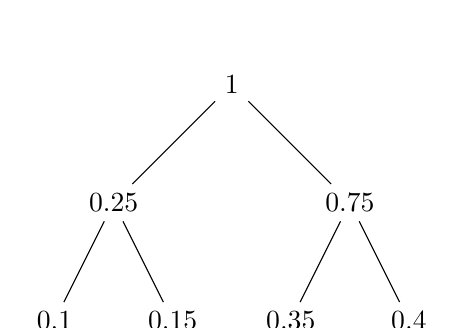
\begin{tikzpicture}
        [   grow = down
        ,   level/.style =
            {   sibling distance = 3cm/#1
            ,   level distance = 1.5cm
            }
        ]
        \node {1}
        child
        {   node {0.25}
            child
            {   node {0.1}
            }
            child
            {   node {0.15}
            }
        }
        child
        {   node {0.75}
            child
            {   node {0.35}
            }
            child
            {   node {0.4}
            }
        };
    \end{tikzpicture}
\end{center}
Suppose the value $r = 0.45$ is randomly generated from a uniform distribution:
$r$ is greater than the left child node, $0.25$, so subtract the left node value
and move to the right child node, $r \leftarrow r - 0.25 = 0.2$;
$r$ is less than the left child node, $0.35$, so move to the left child node;
no left child node is present, search complete;
search ended on the $3^\text{rd}$ child node, select the $3^\text{rd}$
experience from the replay memory.

    \chapter{Python Script for Dueling Double Deep Q-Network}

Full source code, including unused files, can be found at
\url{https://github.com/RanfordS/2020-Masters-Project}.

\inputminted%
[   frame = lines
,   framesep = 2mm
,   mathescape
,   linenos
]{python}{../Code/RLChain/AllDeepQLearning.py}

\end{appendices}
%\begin{center}\import{../Code/}{CharacterRecognitionResults.pgf}\end{center}
%\begin{center}
%    \begin{tikzpicture}
    \loaddata{../Code/CharacterRecognition/FigrFlat.txt}
    \foreach\posx/\posy/\pred/\cert/\actu in \loadeddata
    {   \pgfmathtruncatemacro{\indx}{5*\posy+\posx}
        \node[draw] (N\indx) at (3*\posx,-3.8*\posy)
        {\includegraphics[width=1.5cm]{CRResults/img\indx}};
        \node (P\indx) at (N\indx.north) [anchor=south]
        {\scriptsize Predicted: \pred};
        \node (A\indx) at (P\indx.north) [anchor=south,outer sep=0,inner sep=0]
        {\scriptsize Was: \actu};
        \node (S\indx) at (N\indx.south) [anchor=north]
        {\scriptsize \ifnum \actu=\pred
                Correct
            \else
                \underline{\textbf{Incorrect}}
            \fi};
        \node (C\indx) at (S\indx.south) [anchor=north,outer sep=0,inner sep=0]
        {\scriptsize Certainty: \cert};
    }
\end{tikzpicture}

%\end{center}


\printbibliography

\end{document}
